\documentclass[openany]{tietreport}  % openany: no blank pages before chapters

% Import images
\usepackage{graphicx}
\graphicspath{{figures/}}   % all diagram and screenshot files live in figures/

% Additions to the official template (no layout changes):
\usepackage[figuresright]{rotating}  % sidewaysfigure: wide UML diagrams on a rotated float page
\usepackage{array}    % ragged-right table columns (L)
\newcolumntype{L}[1]{>{\raggedright\arraybackslash}p{#1}}
\usepackage{placeins}  % \FloatBarrier: keep screenshots inside their subsection

% Bibliography configuration (unchanged from the official template)
\usepackage[
  date=year,
  style=alphabetic,
  backend=biber,
  sorting=nty,
  maxnames=5,
  minnames=3,
  maxalphanames=4,
  minalphanames=3,
  backref=true,
  doi=false,
  isbn=false,
  url=false,
  eprint=false
]{biblatex}
\addbibresource{references.bib}
% let long URLs in online references break across lines
\setcounter{biburlnumpenalty}{9000}
\setcounter{biburllcpenalty}{7000}
\setcounter{biburlucpenalty}{8000}

% Only affects paragraphs that would otherwise overflow the margin
\emergencystretch=1.5em

%% ==================================================
%% DIAGRAM PLACEHOLDERS
%% ==================================================
%% \diagram[<max width>]{<file name>}{<what to upload>}{<max height>}
%% If figures/<file name> exists it is inserted automatically;
%% otherwise a framed placeholder box is drawn so the report
%% still compiles. To add a diagram, save the image in the
%% figures/ folder under the exact file name below. No code
%% change is needed.
\newcommand{\diagram}[4][\linewidth]{%
  \IfFileExists{figures/#2}{%
    \includegraphics[width=#1,height=#4,keepaspectratio]{#2}%
  }{%
    \fbox{\parbox[c][#4][c]{0.92#1}{\centering
      \textbf{UPLOAD #3 HERE}\\[0.6em]
      Save the image as \texttt{figures/\detokenize{#2}}}}%
  }%
}

%% FASTER COMPILES ON OVERLEAF (free plan):
%% while editing one chapter, uncomment the line below and list only
%% that chapter. Page and figure numbers of the other chapters are kept.
%% Comment it out again before the final compile.
% \includeonly{chapters/ch3_results}

%% ==================================================
%% PROJECT FIELDS
%% ==================================================

% Course/Lab header
\TitlePageHeader{%
  UCS503 - Software Engineering Project%
}

% Main project title
\ProjectTitle{%
  TravelSync%
}

% Subtitle or project description
\ProjectSubTitle{%
  An Intelligent and Collaborative Travel Platform%
}

% Student information (up to 4 students)
\author{%
  \texttt{1024030501} Jiya Gupta \\
  \texttt{1024030510} Himani Nayyar \\
  \texttt{1024030520} Shreya \\
  \texttt{1024030524} Molika Goela%
}

% Group number, degree, year, program
\TitlePageSubText{%
  Group: \texttt{3C34} BE Third Year, COE%
}

% Faculty advisor/guide name
\AdvisorName{%
  Dr. Nisha Thakur%
}

% Evaluation period and department info
\TitlePageFooterText{{%
    \large End-Semester Evaluation \\[0.2cm]
    \bfseries Computer Science and Engineering
    Department%
  } \\[0.15cm]
  Thapar Institute of Engineering and Technology,
  Patiala%
}

%% ==================================================

\begin{document}

% Generate title page
\maketitle

% Table of contents (auto-generated from chapters)
\tableofcontents

% ===== CHAPTER 1: INTRODUCTION =====

\chapter{Introduction}

\section{Background and Context}

Planning a trip typically requires a traveller to move between many
disconnected services: one source for destination ideas, another for
attractions, another for accommodation, a weather service, a map, and
separate sources for health and safety advisories. When the trip is planned
with friends or family, the group usually adds a messaging application and a
shared spreadsheet to compare options and reach a decision, while tickets and
booking confirmations remain scattered across e-mail inboxes and files. The
result is a planning process that is time-consuming, fragmented and difficult
to personalise.

TravelSync is a web application that brings these activities into a single
platform for travel within India. It serves two kinds of travellers. A
traveller who already knows the destination can select it directly and move
straight to exploring and preparing for it. A traveller who is undecided can
instead describe what the trip should offer, namely travel interests, the
importance of each interest, traveller type, trip duration, total budget,
starting location and the maximum distance they are willing to travel, and
receive a ranked list of destinations that are both similar to these
preferences and practically feasible.

Once a destination is chosen it becomes a \emph{trip}, and every other
module of the platform is organised around that trip: the five top places at
the destination, a smart packing list that adapts to the weather forecast,
accommodation recommendations near the places the traveller intends to visit,
destination-specific health and safety information, an interactive map with
driving distances, and a store for bookings and tickets. A Collaborative
Travel Hub lets a group create a shared space, chat in real time, suggest
destinations, vote, and lock in a final decision that can be converted
directly into a trip. A floating TravelSync assistant answers travel questions
from the platform's own data throughout the application.

\subsection{Problem Statement}

Existing travel-planning workflows are scattered across multiple platforms
and are rarely personalised enough to be genuinely useful. Specifically:

\begin{itemize}
  \item Travellers who are unsure where to go usually have implicit
    constraints, such as budget, duration and acceptable travel distance,
    but no single tool converts these constraints together with their
    interests into a ranked and comparable set of destination options.
  \item General-purpose recommendation lists rarely consider a traveller's
    interests, traveller type, trip duration, budget and starting location
    at the same time.
  \item Information needed once a destination is chosen, such as places to
    visit, accommodation, weather and health advisories, is distributed
    across different services instead of being available in one place.
  \item Packing is handled with generic checklists that do not account
    together for the destination's climate and terrain, the trip length and
    the forecast for the actual travel dates.
  \item Groups travelling together lack a structured way to propose
    destinations, discuss them and reach a collective decision, and fall
    back on separate communication tools.
  \item Bookings, tickets and records of past trips are spread across
    e-mails, files and applications rather than being attached to the trip
    or group they belong to.
\end{itemize}

TravelSync addresses these problems by combining a content-based
recommendation engine with deterministic feasibility constraints,
consolidated destination information, trip-preparation tools, real-time group
collaboration with voting, and booking and travel-history management within
one secure, account-based platform.

\subsection{Existing Systems and Proposed System}

Travellers today rely on several categories of existing systems, each of
which solves part of the problem. Online travel agencies and hotel
aggregators are optimised for booking transport and accommodation once a
destination is already known; they do not help an undecided traveller choose
where to go. Map and review platforms describe places in detail but treat
each destination in isolation. Weather services, public-health advisories
and packing checklists are separate tools, and group decisions are typically
made in general-purpose messaging applications in which suggestions, votes
and the final decision are lost in the conversation history.

The proposed system differs from these in three ways. First, it supports the
\emph{undecided} traveller with an explainable, content-based recommender
\cite{lops2011content} that ranks destinations by similarity to the
traveller's interests and then applies duration, budget and distance
constraints. Second, it makes the trip the central object: every supporting
module (places, packing, stays, health, map and bookings) reads its context
from the saved trip, so the traveller never re-enters the destination, dates
or budget. Third, it treats group planning as a first-class workflow, with
structured destination suggestions, one vote per member, live updates and an
owner-confirmed decision that becomes a shared trip.

\section{Project Objectives}
\label{sec:objectives}

\begin{enumerate}
  \item \textbf{Objective 1:} Build an intelligent trip planner that lets a
    user either select a known destination or obtain a ranked list of up to
    ten recommended destinations from a dataset of 250 Indian destinations,
    using weighted nearest-neighbour similarity over twelve interest features
    and four traveller types, combined with duration, budget and
    great-circle distance constraints.
  \item \textbf{Objective 2:} Consolidate the information and preparation a
    chosen destination needs into a single trip workspace: the top five
    places, a weather-aware packing list, scored accommodation
    recommendations, destination-specific health and safety information and
    an interactive map with driving distances.
  \item \textbf{Objective 3:} Provide a Collaborative Travel Hub in which
    groups of travellers can join through an invite code, chat in real time,
    suggest destinations, vote, and confirm a final destination that is
    converted into a trip for the group.
  \item \textbf{Objective 4:} Support trip management end to end, through
    bookings and tickets with private file attachments, a record of upcoming
    and previous trips, in-app notifications and a conversational travel
    assistant, while protecting every user's data with secure authentication
    and per-user authorisation.
\end{enumerate}

These objectives were framed to be Specific, Measurable, Achievable, Relevant
and Time-bound (SMART). Each objective maps to concrete modules and API
endpoints described in Chapter~\ref{chap:methodology}, each is verified by
automated tests reported in Chapter~\ref{chap:results}, and all four were
delivered within the semester's development window (August to November
2026).

\subsection{Scope of the Project}

The scope of TravelSync is domestic travel within India. The destination
dataset covers 250 destinations, the places dataset contains the top five
places for each of them (1{,}250 places), and 258 starting locations are
available for distance calculations. The following capabilities are in
scope: account management; known-destination selection and preference-based
recommendation; trip creation, editing and deletion; the top places of each
destination; packing lists; accommodation recommendations; health and safety
information; group collaboration; bookings with file attachments; an
interactive map; notifications; and the travel assistant.

The following are deliberately out of scope. TravelSync does not book or pay
for transport or accommodation; bookings are records that the user enters.
It does not display live hotel prices or availability, because the
accommodation data source does not provide them. Its health module provides
general travel awareness only and does not offer medical advice or a
``safe to travel'' score. There is no administrator interface; the curated
datasets are maintained by the development team as versioned files in the
repository.

Development followed the time-to-value order set out in the project
proposal. The core discovery workflow (known-destination selection and
recommendation) was delivered first, followed by the trip workspace and its
supporting modules (top places, packing, stays and health), then the
Collaborative Travel Hub with voting, and finally bookings, the interactive
map and the travel assistant.

\subsection{Software Requirements Specification}

The requirements below follow the structure recommended by IEEE Std 830
\cite{ieee830}. Table~\ref{tab:functional-requirements} lists the functional
requirements and the module that implements each one.

\begin{table}[htbp]
\centering
\begin{tabular}{|l|L{0.56\textwidth}|l|}
  \hline
  \textbf{ID} & \textbf{Functional requirement} & \textbf{Module} \\
  \hline
  FR-01 & Register, log in, log out, change and reset a password & Auth \\
  \hline
  FR-02 & Search the destination dataset and select a known destination
    & Planner \\
  \hline
  FR-03 & Recommend ranked destinations from interests, importance,
    traveller type, duration, budget, start and maximum distance & Planner \\
  \hline
  FR-04 & Save, list, edit (dates, budget, duration) and delete trips
    & Trips \\
  \hline
  FR-05 & Show the top five places of a destination & Places \\
  \hline
  FR-06 & Generate, edit and tick off a packing list; refine it with a
    forecast once dates are set & Packing \\
  \hline
  FR-07 & Recommend, explain, save and remove accommodation for a trip
    & Stays \\
  \hline
  FR-08 & Show current health alerts and historical outbreak patterns for
    the destination's state & Health \\
  \hline
  FR-09 & Create and join groups, chat in real time, suggest destinations,
    vote and confirm a decision & Groups \\
  \hline
  FR-10 & Record personal and group bookings and attach ticket files
    & Bookings \\
  \hline
  FR-11 & Show a trip's places and saved stays on a map with driving
    distances & Map \\
  \hline
  FR-12 & Answer travel questions through a conversational assistant
    & Assistant \\
  \hline
  FR-13 & Notify users of group events and let them mark notifications read
    & Notifications \\
  \hline
\end{tabular}
\caption{Functional requirements}
\label{tab:functional-requirements}
\end{table}

The non-functional requirements are as follows:

\begin{itemize}
  \item \textbf{Security:} passwords are stored only as bcrypt hashes;
    sessions use a signed JWT in an \texttt{httpOnly} cookie; every private
    endpoint verifies that the requested trip, group, booking or file
    belongs to the caller; and state-changing requests from other origins
    are rejected.
  \item \textbf{Reliability:} failures of external providers (accommodation,
    routing, weather and the optional language model) degrade to a clear
    message or a fallback rather than breaking the page, and a database
    outage returns HTTP 503 instead of logging the user out.
  \item \textbf{Performance:} interactive API requests other than
    deliberately slow password hashing should complete well within the
    100\,ms range on a single server process (measured in
    Section~\ref{sec:performance}).
  \item \textbf{Usability and accessibility:} validation errors are shown
    next to the field concerned, live regions announce results to screen
    readers, and the interface adapts to desktop and mobile widths.
  \item \textbf{Maintainability:} the backend is split into routers,
    services and models, every rule-based engine is a pure, unit-tested
    function, and configuration is supplied only through environment
    variables.
  \item \textbf{Transparency:} recommendation and accommodation scores are
    explained to the user, estimated prices are labelled as estimates, and
    health information is labelled as historical, not predictive.
\end{itemize}

The software required to build and run the system is Python 3.10 or later
with the packages listed in \texttt{backend/requirements.txt}; Node.js
22.12 or later for the frontend build and test tool chain; MongoDB (a local
server or MongoDB Atlas); and a current web browser. Optional components are
a Geoapify API key for accommodation and driving distances, an SMTP server
for password recovery, and an OpenAI-compatible chat API key for the
assistant's fallback answers. No special hardware is required: the
measurements in Chapter~\ref{chap:results} were taken on a standard laptop,
and the client runs in any modern desktop or mobile browser.

% ===== CHAPTER 2: METHODOLOGY & DESIGN =====

\chapter{Methodology and Design}
\label{chap:methodology}

\section{System Architecture}

TravelSync was developed with an iterative and incremental process
\cite{sommerville2016}. Each increment delivered one working feature slice,
covering its API endpoints, service logic, user interface and automated
tests, and was integrated into the shared GitHub repository through feature
commits and pull requests. The backend was first prototyped in Flask in late
August 2026 and was migrated to FastAPI \cite{fastapi} immediately afterwards
so that the application could use asynchronous database access, declarative
request validation and native WebSocket support. Later increments added the
packing assistant (September), the health and safety module (October), top
places, stays and the trip workspace (October), real-time group chat and the
assistant (November), and finally bookings, the interactive map and trip
editing (November).

The resulting system follows a layered client--server architecture. A React
single-page application runs in the browser and communicates with a FastAPI
backend through a JSON REST API and, for group chat, a WebSocket connection.
The backend is organised into routers (HTTP and WebSocket endpoints),
services (business logic and the recommendation, packing, health and stay
engines) and models (request validation), with cross-cutting security code
kept in a separate core package. Persistent data is stored in MongoDB through
the asynchronous Motor driver, while curated datasets are shipped with the
backend as versioned CSV and JSON files.

\subsection{High-Level Design}
\label{sec:high-level-design}

Figure~\ref{fig:architecture} shows the major components and their
interactions. Every browser request passes through a fixed middleware chain
before reaching a router: CORS handling restricted to the configured
frontend origins, an Origin/Referer check that rejects state-changing
requests from other sites, and a middleware that adds security headers.
Routers authenticate the caller from the session cookie, validate the request
body against a Pydantic model and delegate to a service. Services read and
write MongoDB, consult the bundled datasets, or call an external provider, and
every provider call is wrapped so that a timeout or quota error produces a
clear, user-safe message rather than an unhandled failure.

\begin{figure}[htbp]
\centering
% Pre-rendered from figures/architecture_source.tex (TikZ), so the
% report compiles faster.
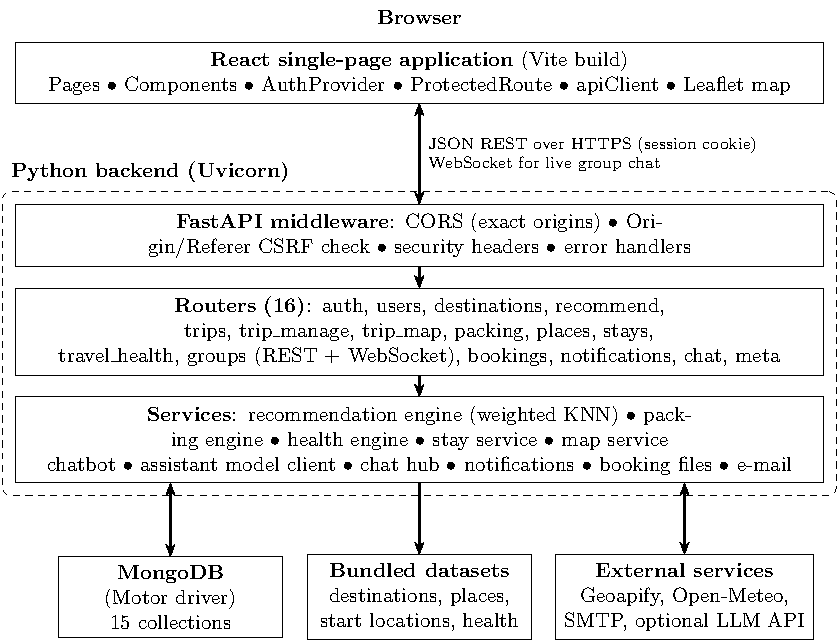
\includegraphics{architecture.pdf}
\caption{High-level architecture of TravelSync}
\label{fig:architecture}
\end{figure}

Real-time collaboration is implemented with the WebSocket protocol
\cite{rfc6455} directly in FastAPI rather than through an additional
messaging service. The socket is receive-only: a chat message is still sent
with an ordinary authenticated \texttt{POST} request, so validation and
membership checks remain in one place, and once the message is stored the
in-process chat hub pushes it to every open socket of that group. The same
channel carries message deletions, read receipts, new suggestions, vote
changes and group decisions.

The actors that interact with the system are the following:

\begin{itemize}
  \item \textbf{Traveller:} registers and logs in, plans trips through
    either known-destination selection or recommendation, and uses the
    packing, stays, health, map, bookings and assistant features for those
    trips.
  \item \textbf{Group Member:} a traveller who has joined a travel group
    through its invite code; reads and sends chat messages, suggests
    destinations, votes, and sees bookings shared with the group. The
    member who created the group is its \emph{owner} and can additionally
    confirm or reopen the group decision and delete the group.
  \item \textbf{External services:} Geoapify \cite{geoapify} supplies
    accommodation listings drawn from OpenStreetMap \cite{haklay2008osm}
    and driving distances; Open-Meteo \cite{openmeteo} supplies weather
    forecasts; OpenStreetMap tile servers supply map tiles directly to the
    browser; an SMTP server delivers password-reset e-mails; and an optional
    OpenAI-compatible chat API answers assistant questions that the built-in
    logic cannot.
\end{itemize}

The mid-semester design included an Administrator actor. During
implementation the team decided not to build an administration interface:
the destination, places and health datasets are curated files maintained in
the repository, which keeps the attack surface smaller and every data change
reviewable through version control.

The UML models and data flow diagrams in the remainder of this section were
produced during the analysis and design phases of the project. They
therefore still show some elements that changed during implementation:
the Administrator actor, and external interfaces whose role became narrower
(weather is used only by the packing assistant, and accommodation comes from
Geoapify with estimated rather than live prices). Where a diagram and the implementation differ, the implementation
described in Section~\ref{sec:implementation} reflects the delivered
system.

\subsubsection{Use Case Diagram}

Figure~\ref{fig:use-case} shows the use case diagram of TravelSync, covering
the Traveller and Group Member actors and the external services on which the
system depends. Each use case corresponds to one or more of the functional
requirements in Table~\ref{tab:functional-requirements}.

% UPLOAD: Use Case Diagram
\begin{figure}[htbp]
  \centering
  % Replace by saving the image as figures/use_case_diagram.jpg
  \diagram{use_case_diagram.jpg}{USE CASE DIAGRAM}{0.75\textheight}
  \caption{TravelSync use case diagram}
  \label{fig:use-case}
\end{figure}

\subsubsection{Use Case Specifications}

Figures~\ref{fig:uc01}--\ref{fig:uc10} document the detailed specification
of the principal use cases shown in Figure~\ref{fig:use-case}, including the
actors, pre-conditions, task sequence and post-conditions of each.

% UPLOAD: Use Case Specification UC-01
\begin{figure}[htbp]
  \centering
  \diagram{uc01_plan_trip.jpg}{UC-01 PLAN TRIP SPECIFICATION}{0.36\textheight}
  \caption{UC-01 -- Plan Trip}
  \label{fig:uc01}
\end{figure}

% UPLOAD: Use Case Specification UC-02
\begin{figure}[htbp]
  \centering
  \diagram{uc02_register_login.jpg}{UC-02 REGISTER / LOGIN SPECIFICATION}{0.36\textheight}
  \caption{UC-02 -- Register / Login}
  \label{fig:uc02}
\end{figure}

% UPLOAD: Use Case Specification UC-03
\begin{figure}[htbp]
  \centering
  \diagram{uc03_view_top_places.jpg}{UC-03 VIEW TOP PLACES SPECIFICATION}{0.36\textheight}
  \caption{UC-03 -- View Top Places at the Destination}
  \label{fig:uc03}
\end{figure}

% UPLOAD: Use Case Specification UC-04
\begin{figure}[htbp]
  \centering
  \diagram{uc04_generate_packing_list.jpg}{UC-04 GENERATE PACKING LIST SPECIFICATION}{0.36\textheight}
  \caption{UC-04 -- Generate a Packing List}
  \label{fig:uc04}
\end{figure}

% UPLOAD: Use Case Specification UC-05
\begin{figure}[htbp]
  \centering
  \diagram{uc05_view_interactive_map.jpg}{UC-05 VIEW INTERACTIVE MAP SPECIFICATION}{0.36\textheight}
  \caption{UC-05 -- View Interactive Map}
  \label{fig:uc05}
\end{figure}

% UPLOAD: Use Case Specification UC-06
\begin{figure}[htbp]
  \centering
  \diagram{uc06_view_recommended_hotels.jpg}{UC-06 VIEW RECOMMENDED HOTELS SPECIFICATION}{0.36\textheight}
  \caption{UC-06 -- View Recommended Hotels}
  \label{fig:uc06}
\end{figure}

% UPLOAD: Use Case Specification UC-07
\begin{figure}[htbp]
  \centering
  \diagram{uc07_health_safety.jpg}{UC-07 HEALTH \& SAFETY SPECIFICATION}{0.36\textheight}
  \caption{UC-07 -- Travel Health \& Safety Warnings}
  \label{fig:uc07}
\end{figure}

% UPLOAD: Use Case Specification UC-08
\begin{figure}[htbp]
  \centering
  \diagram{uc08_group_trip_collaboration.jpg}{UC-08 GROUP TRIP COLLABORATION SPECIFICATION}{0.36\textheight}
  \caption{UC-08 -- Group Trip Collaboration}
  \label{fig:uc08}
\end{figure}

% UPLOAD: Use Case Specification UC-09
\begin{figure}[htbp]
  \centering
  \diagram{uc09_manage_bookings.jpg}{UC-09 MANAGE BOOKINGS SPECIFICATION}{0.36\textheight}
  \caption{UC-09 -- Manage Travel Bookings and Tickets}
  \label{fig:uc09}
\end{figure}

% UPLOAD: Use Case Specification UC-10
\begin{figure}[htbp]
  \centering
  \diagram{uc10_travel_assistant.jpg}{UC-10 TRAVEL ASSISTANT SPECIFICATION}{0.36\textheight}
  \caption{UC-10 -- Interact with Travel Chatbot}
  \label{fig:uc10}
\end{figure}

\subsubsection{Activity Diagram}

Figure~\ref{fig:activity} traces the end-to-end flow of a traveller through
TravelSync: registration and login, the decision between selecting a known
destination and requesting ranked recommendations, retrieval of the
destination's information, the optional packing list, the interactive map,
the branch for group travel (creating or joining a group, discussing and
voting, and confirming the group destination), and finally bookings and the
travel history. The assistant runs in parallel with the whole session.

% Activity Diagram
\begin{figure}[htbp]
  \centering
  \diagram{activity_diagram.jpg}{ACTIVITY DIAGRAM}{0.8\textheight}
  \caption{TravelSync activity diagram}
  \label{fig:activity}
\end{figure}

\subsubsection{Swimlane Diagram}

Figure~\ref{fig:swimlane} presents the same workflow as a swimlane diagram,
assigning each activity to the lane responsible for it: the traveller, the
TravelSync system and the machine-learning module. It makes the hand-offs
between the user interface, the backend and the recommendation engine
explicit.

% Swimlane Diagram
\begin{figure}[htbp]
  \centering
  \diagram{swimlane_diagram.jpg}{SWIMLANE DIAGRAM}{0.8\textheight}
  \caption{TravelSync swimlane diagram}
  \label{fig:swimlane}
\end{figure}

\subsubsection{Sequence Diagram}

Figure~\ref{fig:sequence} presents the messages exchanged between the user,
the frontend, the backend and the database during a typical session: login
and session creation, recommendation and saving of a trip, preparation of
the trip (packing list, stay and health information), synchronisation of
group chat and shared suggestions, a question to the travel assistant, and
retrieval of the travel history.

% Sequence Diagram
\begin{figure}[htbp]
  \centering
  \diagram{sequence_diagram.jpg}{SEQUENCE DIAGRAM}{0.78\textheight}
  \caption{TravelSync sequence diagram}
  \label{fig:sequence}
\end{figure}

\subsubsection{Collaboration Diagram}

Figure~\ref{fig:collaboration} shows the same interaction from the point of
view of the participating objects: the user, the frontend, the backend and
the database. The numbered messages on each link (login, trip discovery and
creation, trip preparation, group collaboration, the assistant query and the
travel history) give the order in which the objects collaborate. Because the
diagram is wide, it is printed on a rotated page.

% Collaboration Diagram (printed rotated on its own page)
\begin{sidewaysfigure}
  \centering
  \diagram[\textheight]{collaboration_diagram.jpg}{COLLABORATION DIAGRAM}{0.82\textwidth}
  \caption{TravelSync collaboration diagram}
  \label{fig:collaboration}
\end{sidewaysfigure}

\subsubsection{Class Diagram}

Figure~\ref{fig:class} shows the UML class diagram of TravelSync, with the
user, trip, destination, group, message, packing list, packing item, booking
and related classes, their attributes and operations, and the associations,
aggregations and compositions between them. The persistent classes
correspond to the MongoDB collections described in
Section~\ref{sec:database-design}, while destinations and places are served
from the curated datasets.

% Class Diagram (printed rotated on its own page)
\begin{sidewaysfigure}
  \centering
  \diagram[\textheight]{class_diagram.jpg}{CLASS DIAGRAM}{0.82\textwidth}
  \caption{TravelSync UML class diagram}
  \label{fig:class}
\end{sidewaysfigure}

\subsubsection{Component and Deployment Diagrams}

Figure~\ref{fig:component} shows the main software components and their
interfaces: the web frontend calls the backend API through its REST
interface; the backend uses the recommendation and health-insight
component, reads and writes the TravelSync database, and fetches data from
external services; and the group chat component delivers chat messages,
suggestions and votes over WebSockets.

% Component Diagram
\begin{figure}[htbp]
  \centering
  \diagram{component_diagram.jpg}{COMPONENT DIAGRAM}{0.32\textheight}
  \caption{TravelSync UML component diagram}
  \label{fig:component}
\end{figure}

Figure~\ref{fig:deployment} shows the target deployment topology: the
static React build is served from a frontend host, the client's web browser
loads it and calls the REST API, a Python/FastAPI application server hosts
the backend API together with the recommendation engine, packing engine,
health engine and group chat server, and the database server runs MongoDB
Atlas. The application server is the only node that contacts the external
APIs.

% Deployment Diagram
\begin{figure}[htbp]
  \centering
  \diagram{deployment_diagram.jpg}{DEPLOYMENT DIAGRAM}{0.36\textheight}
  \caption{TravelSync UML deployment diagram}
  \label{fig:deployment}
\end{figure}

\subsubsection{Data Flow Diagrams}

Figure~\ref{fig:dfd0} shows the context-level (Level~0) data flow diagram, in
which TravelSync is a single process exchanging data with its users and
external data sources. Figure~\ref{fig:dfd1} decomposes the system into eight
processes: 1.0 Authenticate and Manage User, 2.0 Recommend Destination,
3.0 Plan and Manage Trip, 4.0 Manage Group Trip, 5.0 Provide Travel
Recommendations, 6.0 Generate Smart Packing Checklist, 7.0 Travel
Assistant/Chatbot and 8.0 Manage Bookings and Trip History.
Figures~\ref{fig:dfd2-p1}--\ref{fig:dfd2-p8} refine each of these processes
into its Level~2 sub-processes and the data stores they use. The Level~1
diagram is printed on a rotated page.

% Level 0 Data Flow Diagram
\begin{figure}[htbp]
  \centering
  \diagram{dfd_level0.jpg}{LEVEL 0 DATA FLOW DIAGRAM}{0.4\textheight}
  \caption{Level 0 (context) data flow diagram}
  \label{fig:dfd0}
\end{figure}

% Level 1 Data Flow Diagram (printed rotated on its own page)
\begin{sidewaysfigure}
  \centering
  \diagram[\textheight]{dfd_level1.jpg}{LEVEL 1 DATA FLOW DIAGRAM}{0.82\textwidth}
  \caption{Level 1 data flow diagram}
  \label{fig:dfd1}
\end{sidewaysfigure}

% Level 2 Data Flow Diagrams
\begin{figure}[htbp]
  \centering
  \diagram{dfd_level2_p1.jpg}{LEVEL 2 DFD -- PROCESS 1.0}{0.38\textheight}
  \caption{Level 2 DFD -- Process 1.0: Authenticate and Manage User}
  \label{fig:dfd2-p1}
\end{figure}

\begin{figure}[htbp]
  \centering
  \diagram{dfd_level2_p2.jpg}{LEVEL 2 DFD -- PROCESS 2.0}{0.38\textheight}
  \caption{Level 2 DFD -- Process 2.0: Recommend Destination}
  \label{fig:dfd2-p2}
\end{figure}

\begin{figure}[htbp]
  \centering
  \diagram{dfd_level2_p3.jpg}{LEVEL 2 DFD -- PROCESS 3.0}{0.38\textheight}
  \caption{Level 2 DFD -- Process 3.0: Plan and Manage Trip}
  \label{fig:dfd2-p3}
\end{figure}

\begin{figure}[htbp]
  \centering
  \diagram{dfd_level2_p4.jpg}{LEVEL 2 DFD -- PROCESS 4.0}{0.38\textheight}
  \caption{Level 2 DFD -- Process 4.0: Manage Group Trip}
  \label{fig:dfd2-p4}
\end{figure}

\begin{figure}[htbp]
  \centering
  \diagram{dfd_level2_p5.jpg}{LEVEL 2 DFD -- PROCESS 5.0}{0.38\textheight}
  \caption{Level 2 DFD -- Process 5.0: Provide Travel Recommendations}
  \label{fig:dfd2-p5}
\end{figure}

\begin{figure}[htbp]
  \centering
  \diagram{dfd_level2_p6.jpg}{LEVEL 2 DFD -- PROCESS 6.0}{0.38\textheight}
  \caption{Level 2 DFD -- Process 6.0: Generate Smart Packing Checklist}
  \label{fig:dfd2-p6}
\end{figure}

\begin{figure}[htbp]
  \centering
  \diagram{dfd_level2_p7.jpg}{LEVEL 2 DFD -- PROCESS 7.0}{0.38\textheight}
  \caption{Level 2 DFD -- Process 7.0: Travel Assistant / Chatbot}
  \label{fig:dfd2-p7}
\end{figure}

\begin{figure}[htbp]
  \centering
  \diagram{dfd_level2_p8.jpg}{LEVEL 2 DFD -- PROCESS 8.0}{0.38\textheight}
  \caption{Level 2 DFD -- Process 8.0: Manage Bookings and Trip History}
  \label{fig:dfd2-p8}
\end{figure}

\FloatBarrier

\subsection{Technical Stack}

\begin{itemize}
  \item \textbf{Framework/Language:} JavaScript with React~19 \cite{react},
    React Router~7 and the Vite~8 build tool for the frontend; Python with
    FastAPI \cite{fastapi}, Pydantic validation and the Uvicorn ASGI server
    for the backend.
  \item \textbf{Database:} MongoDB \cite{mongodb}, accessed asynchronously
    through the Motor driver, used locally during development and through
    MongoDB Atlas for the shared deployment.
  \item \textbf{Machine learning and data:} scikit-learn
    \cite{pedregosa2011sklearn} for feature scaling, Isolation Forest and
    K-Means, together with NumPy and pandas.
  \item \textbf{Security:} bcrypt password hashing \cite{provos1999bcrypt}
    and PyJWT for signed session tokens \cite{rfc7519}.
  \item \textbf{Tools:} Git and GitHub for version control and pull
    requests; pytest \cite{pytest} with pytest-asyncio and mongomock-motor
    for backend tests; Vitest \cite{vitest}, Testing Library and jsdom for
    frontend tests; ESLint for static analysis.
  \item \textbf{Libraries and external services:} Leaflet \cite{leaflet}
    with OpenStreetMap tiles for maps; lucide-react for icons; HTTPX for
    outgoing HTTP calls; the Geoapify Places and Route Matrix APIs
    \cite{geoapify}; the Open-Meteo forecast API \cite{openmeteo}; the
    browser Geolocation API; and, optionally, any OpenAI-compatible chat
    completion API for the assistant.
\end{itemize}

Table~\ref{tab:api} summarises the REST API exposed by the sixteen routers.
All paths are prefixed with \texttt{/api}; every route except the public
metadata, destination search, places and authentication routes requires a
valid session.

\begin{table}[htbp]
\centering
\begin{tabular}{|L{0.34\textwidth}|L{0.58\textwidth}|}
  \hline
  \textbf{Base path} & \textbf{Main operations} \\
  \hline
  \texttt{/auth} & signup, login, logout, current user, change password,
    recovery status, forgot and reset password \\
  \hline
  \texttt{/users/me} & read and update profile; read and update settings \\
  \hline
  \texttt{/destinations}, \texttt{/start-locations} & search destinations,
    read one destination profile, search starting locations \\
  \hline
  \texttt{/recommend} & ranked destination recommendations \\
  \hline
  \texttt{/trips} & list, read, create, edit (budget, duration, dates) and
    delete trips \\
  \hline
  \texttt{/trips/\{id\}/packing-list} & read, generate, edit items, set
    dates and refresh forecast \\
  \hline
  \texttt{/trips/\{id\}/stays} & recommendations, saved stays, save and
    remove a stay \\
  \hline
  \texttt{/trips/\{id\}/map} & map data; driving distances from the user \\
  \hline
  \texttt{/places/\{destination\}} & top five places of a destination \\
  \hline
  \texttt{/travel-health/\{dest.\}} & alerts and historical profile for the
    destination's state \\
  \hline
  \texttt{/groups} & create, join, list, read, leave, delete; messages,
    read receipts, unread counts; suggestions, votes, decision; WebSocket
    \texttt{/\{id\}/ws} \\
  \hline
  \texttt{/bookings} & list, create, edit, delete, share to group; upload,
    download and delete files \\
  \hline
  \texttt{/notifications} & list, mark one or all as read \\
  \hline
  \texttt{/chat} & ask the TravelSync assistant \\
  \hline
  \texttt{/health}, \texttt{/features} & service status and feature flags \\
  \hline
\end{tabular}
\caption{Summary of the TravelSync REST API}
\label{tab:api}
\end{table}

\section{Implementation Details}
\label{sec:implementation}

\subsection{Module 1: Core Functionality}

The core of TravelSync consists of secure account management, the
Intelligent Destination Finder, trip management with top places, and the
Smart Packing Assistant. Together they implement Objective~1 and the
trip-workspace part of Objective~2.

\subsubsection{Authentication and Session Management}

New passwords must contain 8 to 72 bytes with at least one uppercase letter,
one lowercase letter, one digit and one special character; the 72-byte limit
exists because bcrypt ignores input beyond that length, and the frontend
mirrors the same policy so that users see the rules as they type. Passwords
are stored only as bcrypt hashes \cite{provos1999bcrypt}. On successful
signup or login the backend issues an HS256-signed JWT \cite{rfc7519}
carrying the user identifier, issue time, a seven-day expiry and a
\emph{token version}, and places it in an \texttt{httpOnly} cookie with the
\texttt{SameSite=Lax} attribute, so that browser scripts can never read it.
Changing or resetting a password increments the stored token version, which
invalidates every token issued earlier and therefore signs the user out on
all other devices.

Several further measures protect the login flow. A failed login for an
unknown e-mail address performs a dummy bcrypt comparison, so the response
time does not reveal whether an account exists, and repeated failures are
throttled (five failures within fifteen minutes by default). State-changing
requests that carry the session cookie must come from a configured frontend
origin, following the OWASP guidance on cross-site request forgery
\cite{owaspcsrf}. Password recovery is offered only when an SMTP server is
configured: a random single-use token is e-mailed, only its SHA-256 hash is
stored, and a MongoDB TTL index deletes it after thirty minutes. In
production mode the application refuses to start with a weak JWT secret,
insecure cookies or a wildcard CORS origin.

\subsubsection{Intelligent Destination Finder}

A traveller who knows the destination searches the 250-destination dataset
by name or state and saves it as a trip directly. An undecided traveller
selects one or more of twelve interests (Mountain, Beach, Nature, Adventure,
Culture, Relaxation, Nightlife, Spiritual, Trekking, Photography, Food and
Heritage), sets the importance of each, chooses a traveller type (Family,
Couple, Friends or Solo), and enters the trip duration, total budget,
starting location and maximum travel distance. The recommendation engine is
a content-based recommender \cite{lops2011content} built on the
nearest-neighbour principle \cite{cover1967knn}:

\[
\begin{array}{c}
\text{User Preferences} \rightarrow \text{Feature Vector} \rightarrow
\text{Weighted KNN} \\[2pt]
\rightarrow \text{Constraint Scoring} \rightarrow
\text{Ranked Recommendations}
\end{array}
\]

Every destination is described by sixteen features: the twelve interest
scores and four traveller-type suitability scores, each between 0 and 1. At
start-up the engine fits a \texttt{StandardScaler} to these columns. For a
request, the user vector $\mathbf{u}$ holds the stated interest preferences
and a one-hot encoding of the traveller type, and the weight vector
$\mathbf{w}$ holds the importance of each interest (0 to 3) with a fixed
weight of 3 on the chosen traveller type. The preference distance and score
of destination $i$ are
\[
  d_i = \sqrt{\sum_{j=1}^{16} w_j\,\bigl(x_{ij} - u_j\bigr)^2},
  \qquad
  s^{\mathrm{pref}}_i = \frac{1}{1 + d_i},
\]
computed on the standardised features. The sixty nearest destinations form
the candidate set, which is then scored against the practical constraints. A
destination whose ideal stay is within one day of the requested duration
receives a duration score of 1.0, decreasing to 0.3 for larger differences.
The estimated trip cost (average daily budget multiplied by the duration)
scores highest when it falls between 85\% and 100\% of the stated budget, is
tolerated with lower scores up to 125\%, and is rejected beyond that. The
great-circle distance from the starting location is computed with the
haversine formula \cite{sinnott1984haversine}; destinations within the
maximum distance score 1.0, those up to 10\% beyond it score 0.75, and the
rest are removed. The final score is
\[
  s_i = 0.60\,s^{\mathrm{pref}}_i + 0.15\,s^{\mathrm{dur}}_i
      + 0.15\,s^{\mathrm{bud}}_i + 0.10\,s^{\mathrm{dist}}_i ,
\]
and the top results (six by default, at most ten) are returned with every
component score, the estimated budget and the distance, so the interface can
show why each destination was chosen. The engine needs no external model
file: everything it requires is in the bundled dataset, which makes the
recommendations reproducible on a fresh installation.

\subsubsection{Trip Management and Top Places}

Choosing a destination, whether from search, from a recommendation or from a
group decision, creates a trip that records the destination, its state,
region and coordinates, the duration, budget, traveller type and the
source of the decision. The \emph{My Trips} page separates upcoming and
previous trips, and each trip opens a trip workspace that summarises its
packing progress, shortlisted stays, health status and bookings. Budget,
duration and travel dates can be edited later; dates must be valid, ordered
and no more than ninety days apart. Deleting a trip removes its packing list,
saved stays and bookings with their files, and never affects another user's
data.

The top five places for every destination are served from a curated dataset
of 1{,}250 places with their category, description and coordinates. These
places are reused by the stays module as location anchors and by the map as
markers.

\subsubsection{Smart Packing Assistant}

The packing assistant is a transparent rule engine rather than a learned
model, so every item can be explained and unit-tested. It works in two
tiers, because exact travel dates are often unknown when planning begins:

\[
\begin{array}{c}
\text{Destination climate and terrain} + \text{Duration} \rightarrow
\text{Tier 1 climate list} \\[2pt]
\xrightarrow{\ \text{dates added}\ }
\text{Open-Meteo forecast} \rightarrow \text{Tier 2 forecast list}
\end{array}
\]

The \emph{climate} tier is always available: it uses the destination's
region and its terrain and activity profile from the dataset to generate
categorised items (clothing, weather, health, electronics, documents and
activity-specific gear), with clothing quantities scaled to the trip length.
When the trip has travel dates within the forecast window, the
\emph{forecast} tier calls the Open-Meteo API \cite{openmeteo}, which needs
no API key, summarises the expected temperatures and rain, and refines the
weather-dependent items. If the forecast service fails, the list falls back
to the climate tier instead of failing. Regenerating a list preserves items
the user added and items already marked as packed, and a unique index on the
trip identifier guarantees that two simultaneous first requests create
exactly one list.

\subsection{Module 2: Secondary Features}

The secondary modules complete Objectives~2 to~4.

\subsubsection{Smart Stay Recommendations}

For a trip, the stay service first builds an \emph{anchor} from the
coordinates of the destination's top five places, falling back to the
destination centre when necessary, and fetches nearby accommodation from the
Geoapify Places API \cite{geoapify}, whose listings come from OpenStreetMap
\cite{haklay2008osm}. Results are cached in MongoDB for seven days per
destination through a TTL index, which keeps usage within the provider's
free quota. Each stay receives a 0--100 match score from four explainable
parts: location (40\%, the average haversine distance to the top five
places), budget (30\%, the estimated price per person against the trip's
nightly budget), traveller fit (20\%, how well the stay type suits the
traveller type) and quality (10\%, star rating and listing completeness).
Each recommendation carries plain-language reasons. Because neither Geoapify
nor OpenStreetMap provides live prices, the price shown is an estimated band
derived from the stay type, star rating and the destination's cost level,
and it is always labelled as an estimate. Users can shortlist stays on a
trip; a unique index on the trip and stay key makes saving idempotent.

\subsubsection{Travel Health and Safety Intelligence}

The health module answers the question ``what has happened here before?''
for the state of the chosen destination, and it is explicitly presented as
historical context rather than a prediction or a safety score. It has two
parts. The first is a short list of current outbreak alerts curated from
official public-health sources, each with its source, severity and
reporting date; an alert is shown as active for 45 days and as an earlier
alert for up to a year, and the absence of an alert is never presented as
evidence of safety. The second part analyses a historical outbreak dataset
stored in the weekly outbreak format of the Integrated Disease Surveillance
Programme \cite{idsp}, containing 33{,}076 outbreak records from 2009 to
2026 across 34 states and union territories. At start-up the health engine
computes:

\begin{itemize}
  \item \textbf{Seasonal patterns:} outbreak counts by calendar month for
    each state and disease group, which the interface can filter by the
    intended travel month.
  \item \textbf{Anomaly detection:} two Isolation Forest models
    \cite{liu2008iforest} with 200 trees each, one flagging state-months
    with unusually high outbreak activity and one flagging individual
    outbreaks that were unusually large for their disease.
  \item \textbf{Clustering:} K-Means \cite{lloyd1982kmeans} over
    standardised per-state profiles (the share of each disease group, the
    log mean case count, the log case-fatality rate and a cyclic encoding of
    the peak month), grouping states with similar historical patterns.
\end{itemize}



\subsubsection{Collaborative Travel Hub}

A user creates a group with a name and description and receives a unique
invite code; others join by entering the code, up to twenty members per
group, with the capacity re-checked atomically to prevent over-filling. Group
chat loads the newest fifty messages and pages back through older ones on
request; new messages, deletions and read receipts arrive live through the
WebSocket described in Section~\ref{sec:high-level-design}, and unread counts
are shown in the navigation. Deleting a message is a soft delete that also
erases its text from the database.

Any member can suggest a destination, optionally with a budget, duration,
note and the interests it fits; the suggestion appears both in the
\emph{Destination ideas \& votes} panel and as a card in the chat. Each
member has exactly one vote, enforced by a unique index on the group and
user, and voting for another idea moves the vote. The owner confirms the
winning suggestion, which closes voting and notifies the other members, and
can reopen voting if the group changes its mind. A confirmed decision can be
turned into a trip whose companions are the group's members.

\subsubsection{Bookings, Tickets and Trip History}

Bookings record hotel, flight, train, bus, activity or other reservations
that the user has made elsewhere; TravelSync does not make, pay for or
confirm bookings. Each booking belongs to exactly one personal trip or one
group. Group bookings are visible to all members and editable only by their
author or the group owner, and a booking can be shared into the group chat
as a card that deliberately omits the reference number, amount and files.

Up to five files of at most 5\,MB each can be attached to a booking. The file
type is determined from the file's first bytes rather than its name or
declared content type, and only PDF, PNG, JPEG and WebP files are accepted.
Files are stored in a dedicated MongoDB collection, have no public URL and
can only be downloaded through an endpoint that checks the caller's access.
Deleting a booking, trip or group removes the related files. Together with
the upcoming and previous trip views, this provides the structured travel
history required by Objective~4.

\subsubsection{Interactive Travel Map}

The trip map is a lazily loaded Leaflet \cite{leaflet} page that draws
OpenStreetMap tiles, the destination centre, the top five places and the
shortlisted stays. With the user's permission, the browser Geolocation API
provides the current position, and the backend requests driving distances
and times from the Geoapify Route Matrix API. To protect privacy and the
free quota, the origin is rounded to two decimal places (about one
kilometre) before it is sent or cached, cached results expire after
twenty-four hours and are keyed only by coordinates (never by user or trip),
and each user is limited to twenty live lookups per hour. If routing is
unavailable, the page falls back to straight-line haversine distances
computed in the browser.

\subsubsection{TravelSync Assistant}

The floating assistant answers questions from TravelSync's own data. It
identifies what a question is about (a destination or state named in the
message, the destination already under discussion, or the user's most
recent trip) and what is being asked by counting keyword matches for
intents such as places, packing, health, recommendations, trips, groups and
destination facts. It then builds the answer from the same services used
elsewhere in the application, with in-app links and suggested follow-up
questions, and it can only ever see the logged-in user's own trips and
groups. If an OpenAI-compatible model is configured, questions that the
built-in logic cannot match are forwarded to it; only the question text is
sent, never the user's name, trips or groups, each user may ask eight such
questions per ten minutes, and any timeout, quota error or empty answer
falls back to the built-in reply.

\subsubsection{Notifications}

In-app notifications are created only by real events, such as a member
joining, a destination being suggested or a decision being confirmed. They
are private to the recipient, shown under a bell icon with an unread count,
and can be marked as read individually or all at once.

\subsection{Database Design}
\label{sec:database-design}

TravelSync uses MongoDB because most of its entities are naturally
document-shaped: a packing list is a list of items, a group holds an array of
member identifiers, and a stay recommendation is cached as the provider
returned it. Relationships are expressed through identifier references, and
the access rules are enforced in the service layer. Table~\ref{tab:collections}
lists the fifteen collections and the indexes that the application creates
at start-up. Index creation is idempotent; if the database is unavailable at
start-up, a background task retries until every index exists, and the
application never deletes user data to make an index build succeed.

\begin{table}[htbp]
\centering
\begin{tabular}{|L{0.25\textwidth}|L{0.36\textwidth}|L{0.29\textwidth}|}
  \hline
  \textbf{Collection} & \textbf{Purpose} & \textbf{Indexes} \\
  \hline
  \texttt{users} & accounts, profile, settings, token version
    & e-mail (unique) \\
  \hline
  \texttt{trips} & saved trips & user, created date \\
  \hline
  \texttt{packing\_lists} & one packing list per trip & trip (unique) \\
  \hline
  \texttt{saved\_stays} & shortlisted stays & trip + stay key (unique) \\
  \hline
  \texttt{stay\_cache} & provider results per destination
    & TTL, 7 days \\
  \hline
  \texttt{map\_distance\_cache} & driving distances & TTL, 24 hours \\
  \hline
  \texttt{password\_resets} & hashed reset tokens
    & token hash (unique), TTL \\
  \hline
  \texttt{groups} & groups, members, owner, decision
    & invite code (unique); member, date \\
  \hline
  \texttt{group\_messages} & chat messages & group, created date \\
  \hline
  \texttt{group\_suggestions} & destination ideas
    & group + destination (unique) \\
  \hline
  \texttt{group\_votes} & one vote per member & group + user (unique) \\
  \hline
  \texttt{group\_reads} & read receipts & group + user (unique) \\
  \hline
  \texttt{bookings} & personal and group bookings
    & user, trip, date; group, date \\
  \hline
  \texttt{booking\_files} & attached files & booking \\
  \hline
  \texttt{notifications} & in-app notifications & user, created date \\
  \hline
\end{tabular}
\caption{MongoDB collections and indexes}
\label{tab:collections}
\end{table}

The relationships between these collections follow the associations of the
class diagram in Figure~\ref{fig:class}: a user owns trips and bookings, a
trip has at most one packing list and any number of saved stays, and a
group references its members and owns its messages, suggestions, votes,
read receipts and group bookings.

\subsection{Frontend Implementation}

The frontend is a React single-page application. Routing is defined in one
place: public routes cover the landing, login, signup and password-recovery
pages, while every other page is wrapped in a \texttt{ProtectedRoute} that
redirects anonymous visitors to the login page. An \texttt{AuthProvider}
context loads the current user from \texttt{/api/auth/me} at start-up and
exposes login, signup and logout to the rest of the application. Logged-in
pages share an application shell with a collapsible sidebar, a destination
search bar, the notifications bell and the floating map and assistant
buttons.

All network access goes through a single \texttt{apiClient} module that sends
requests with the session cookie, converts network failures and the
backend's uniform error format into readable messages, attaches field-level
validation errors to the relevant inputs, and returns the user to the login
page when a session expires. Each feature has a thin service
module (for example \texttt{tripApi}, \texttt{groupApi} and
\texttt{bookingApi}) on top of this client. Group pages open the chat
WebSocket and keep a light polling loop as a fallback, which also catches up
on anything missed after a reconnection. The
Leaflet map is loaded on demand, so its code is not downloaded until a user
opens a map. Forms validate input before sending it, move focus to the
first invalid field, and announce results through ARIA live regions.

\subsection{Application Screens}

Figures~\ref{fig:scr-landing}--\ref{fig:scr-assistant} show the implemented
application. The screens were captured from the running system populated
with the four team accounts, a trip to Manali, the group \emph{Winter
Himachal Trip} and three bookings.

\begin{figure}[htbp]
  \centering
  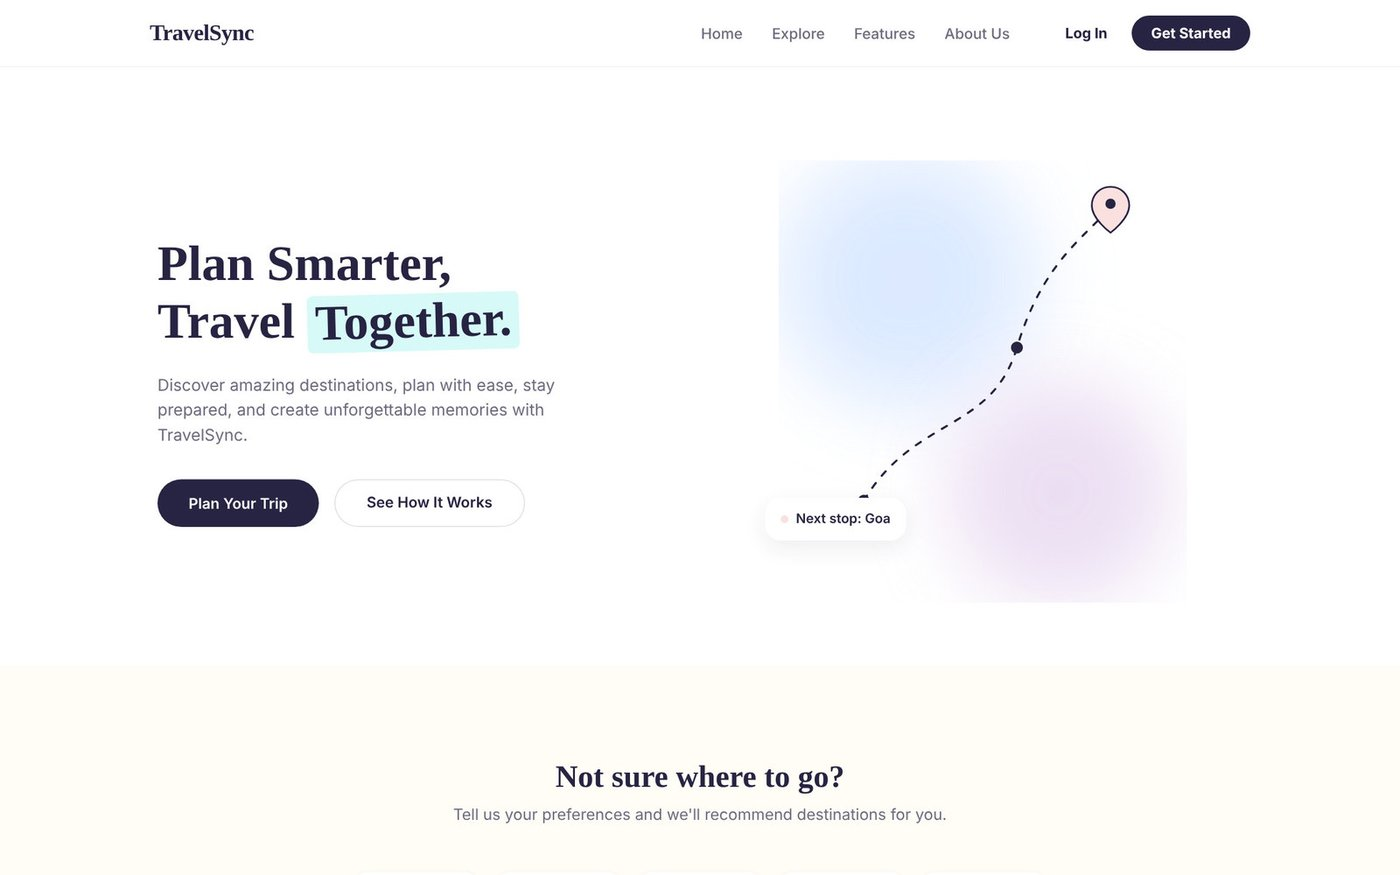
\includegraphics[width=0.9\textwidth]{screenshots/landing_page.jpg}
  \caption{Landing page}
  \label{fig:scr-landing}
\end{figure}

\begin{figure}[htbp]
  \centering
  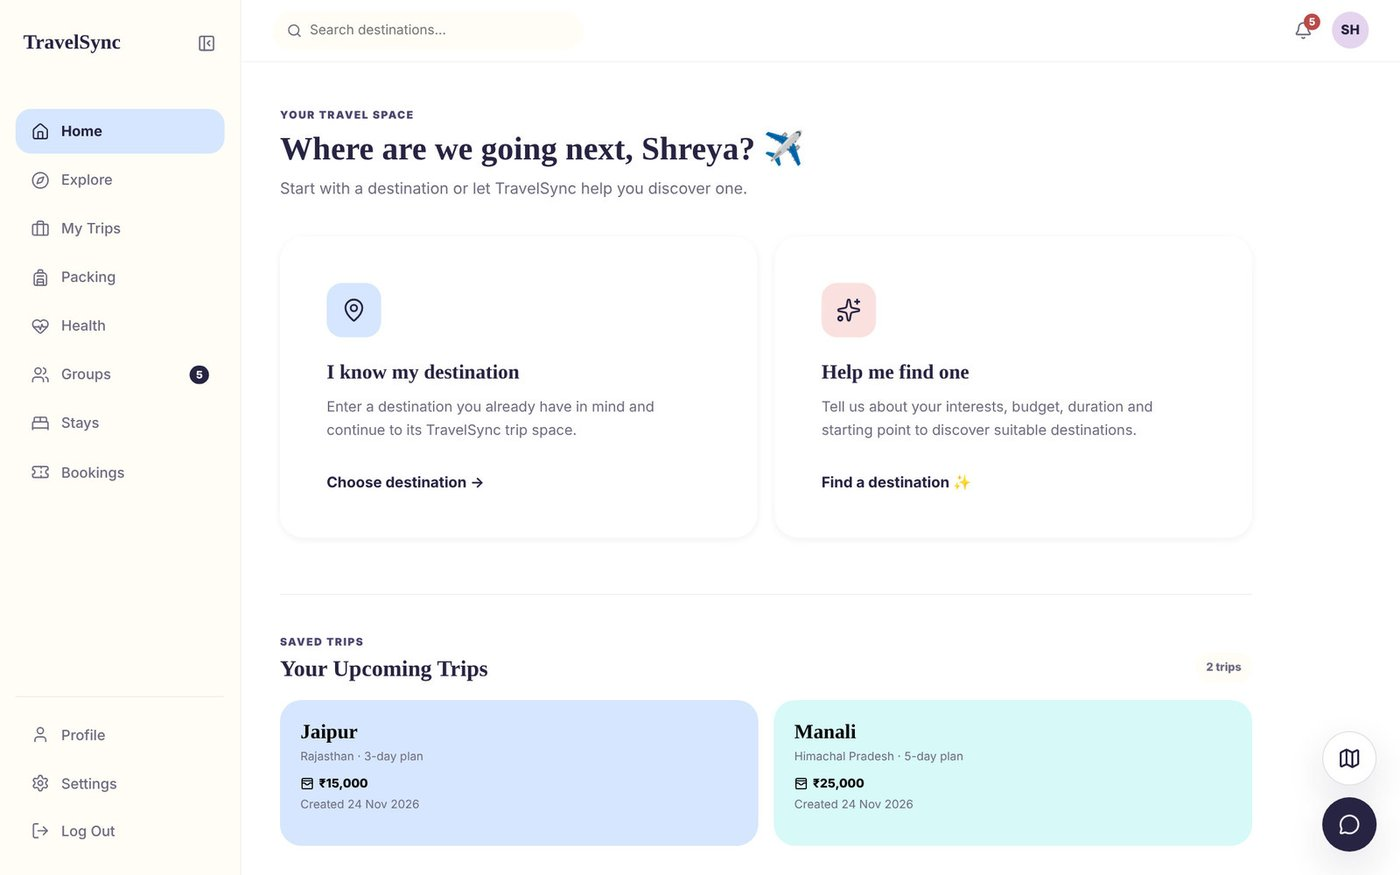
\includegraphics[width=0.9\textwidth]{screenshots/home_dashboard.jpg}
  \caption{Home dashboard with the two planning paths and saved trips}
  \label{fig:scr-home}
\end{figure}

\begin{figure}[htbp]
  \centering
  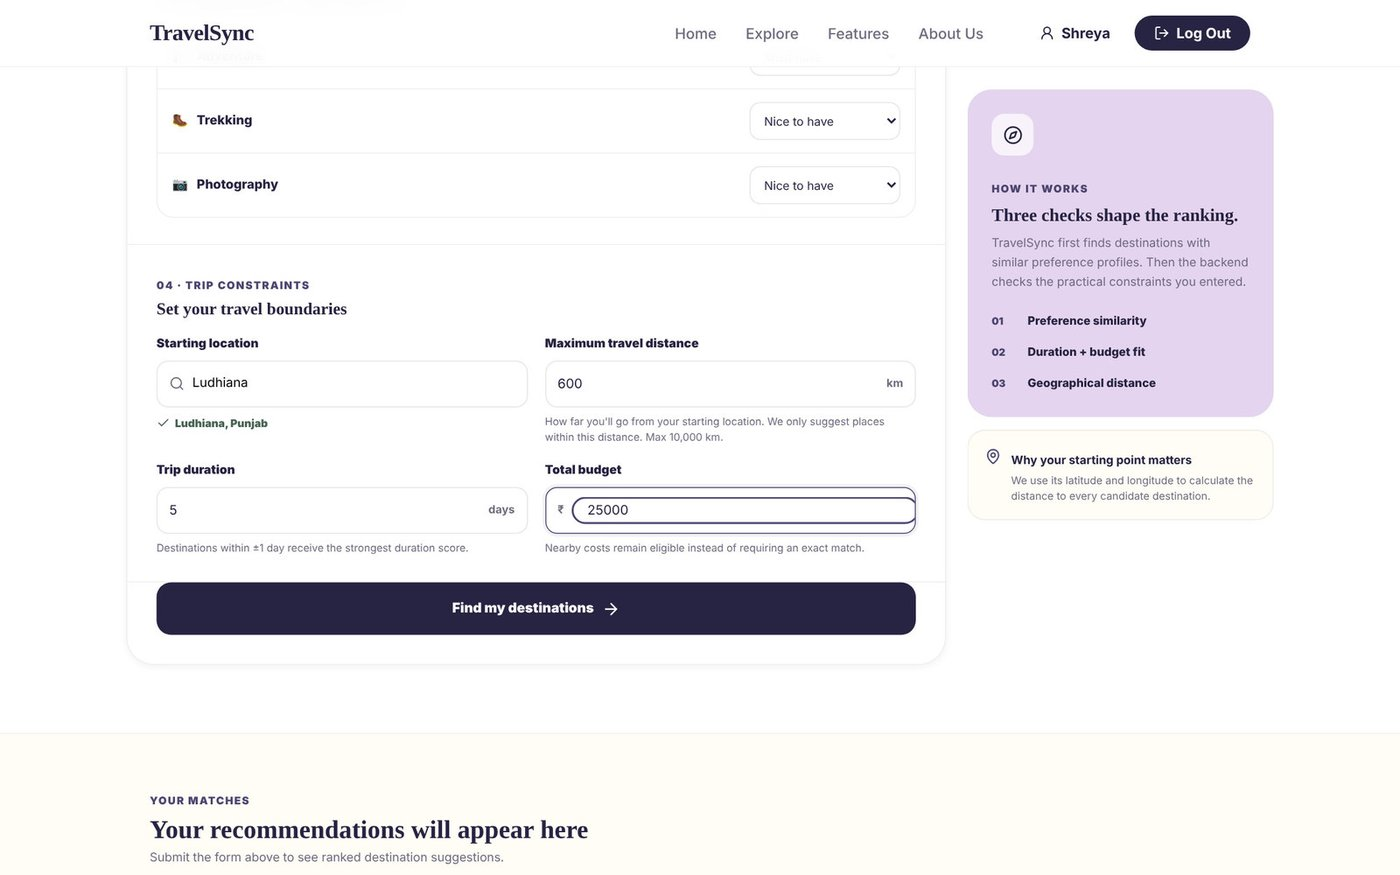
\includegraphics[width=0.9\textwidth]{screenshots/recommendation_form.jpg}
  \caption{Recommendation form: interest priorities and trip constraints}
  \label{fig:scr-rec-form}
\end{figure}

\begin{figure}[htbp]
  \centering
  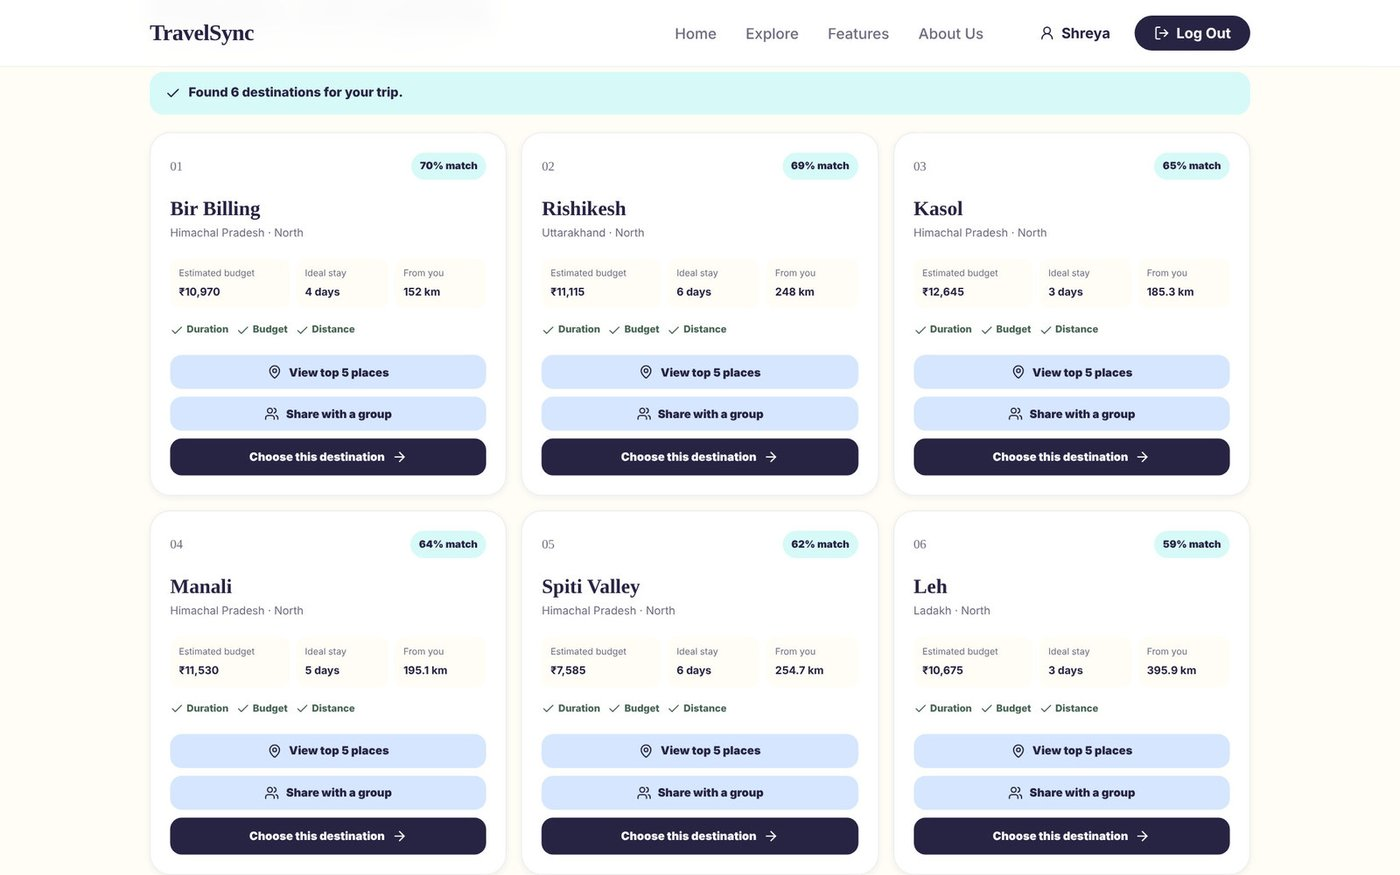
\includegraphics[width=0.9\textwidth]{screenshots/recommendation_results.jpg}
  \caption{Ranked recommendations with match score, budget, stay and
    distance checks}
  \label{fig:scr-rec-results}
\end{figure}

\begin{figure}[htbp]
  \centering
  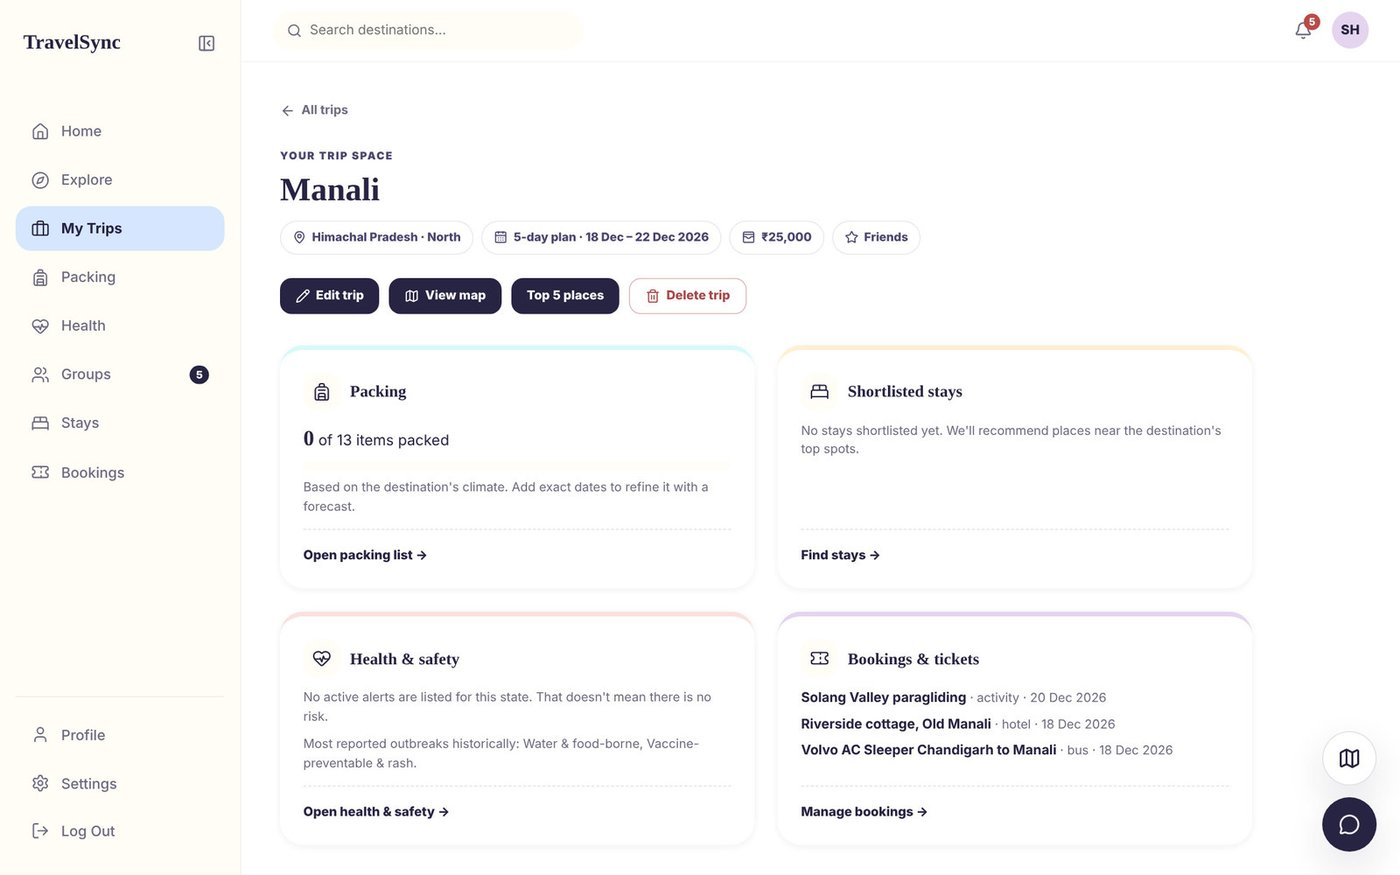
\includegraphics[width=0.9\textwidth]{screenshots/trip_hub.jpg}
  \caption{Trip workspace for a saved trip}
  \label{fig:scr-trip}
\end{figure}

\begin{figure}[htbp]
  \centering
  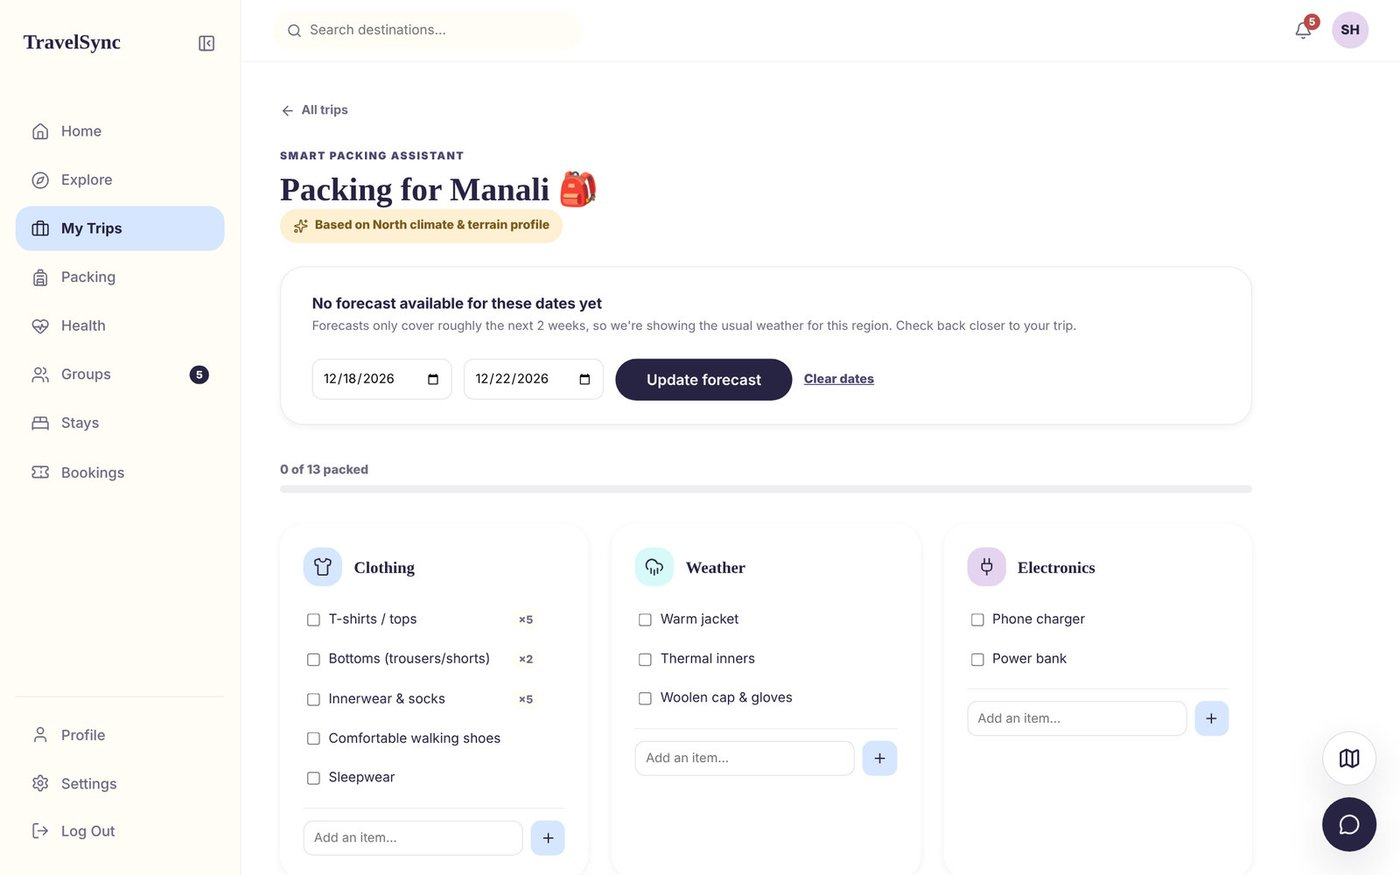
\includegraphics[width=0.9\textwidth]{screenshots/packing_assistant.jpg}
  \caption{Smart Packing Assistant}
  \label{fig:scr-packing}
\end{figure}

\begin{figure}[htbp]
  \centering
  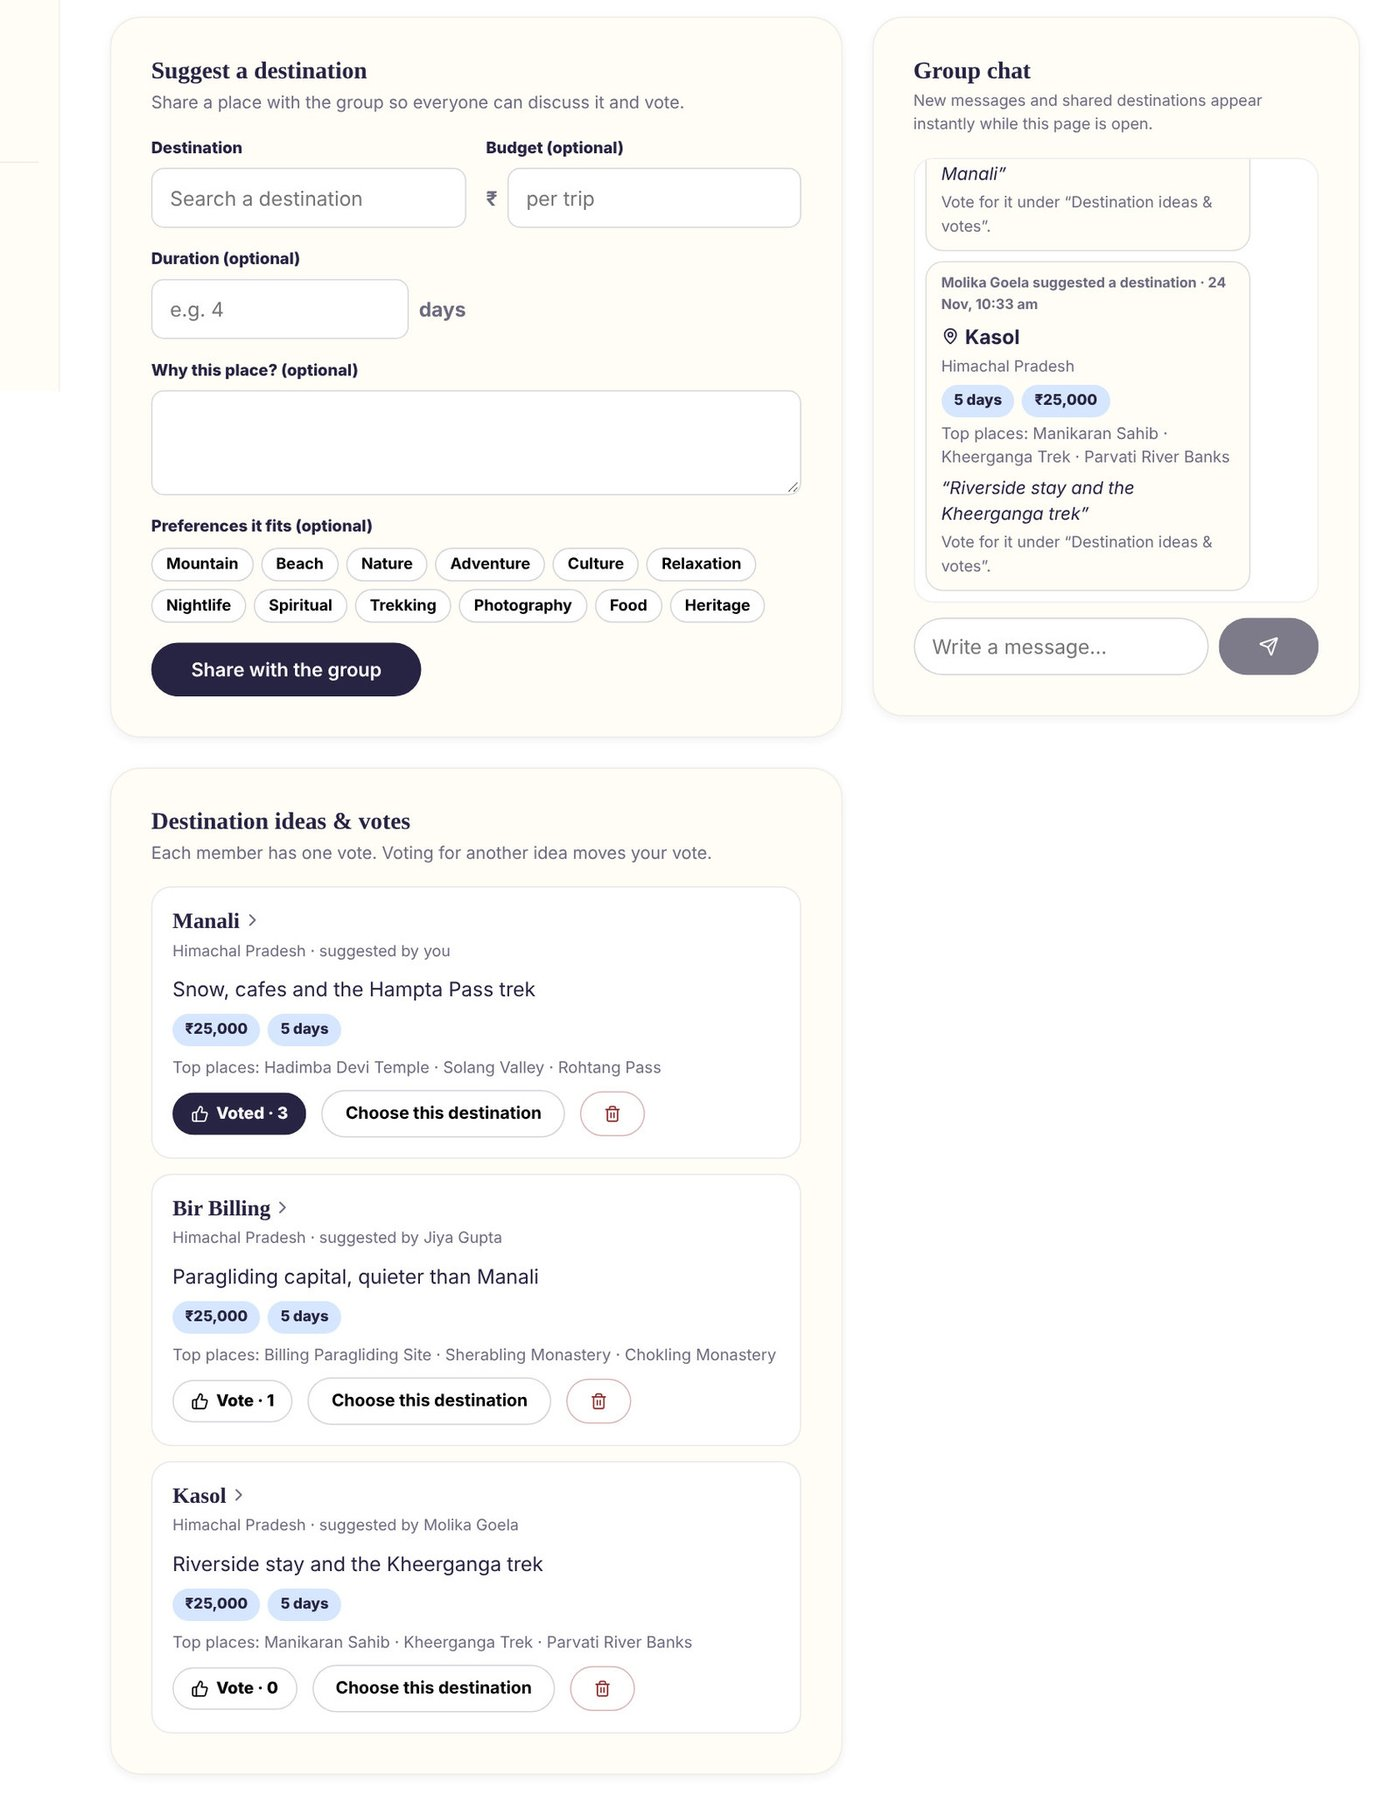
\includegraphics[width=0.82\textwidth]{screenshots/group_collaboration.jpg}
  \caption{Collaborative Travel Hub: destination suggestions, votes and
    group chat}
  \label{fig:scr-group}
\end{figure}

\begin{figure}[htbp]
  \centering
  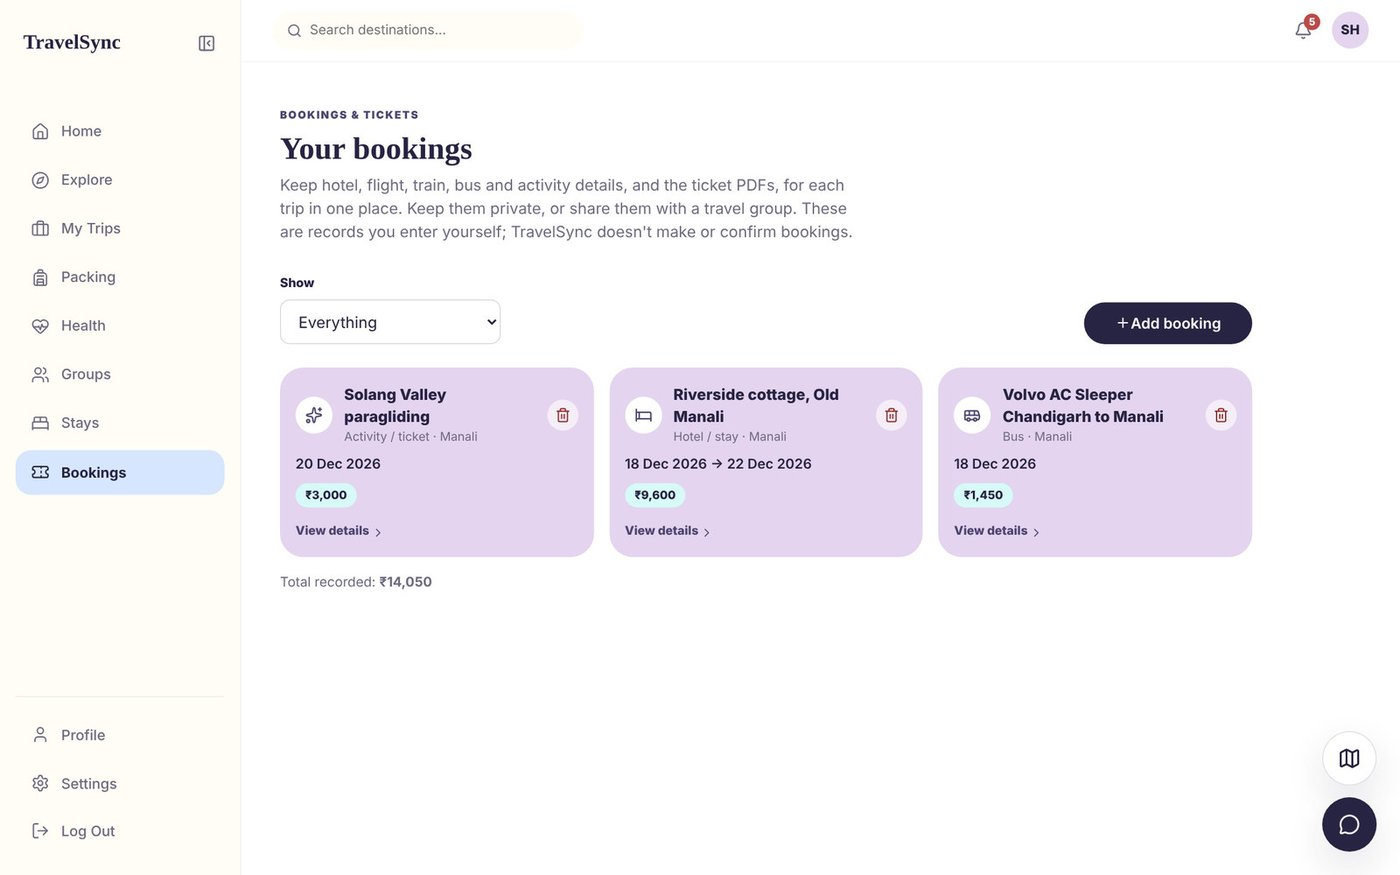
\includegraphics[width=0.9\textwidth]{screenshots/bookings.jpg}
  \caption{Bookings and tickets}
  \label{fig:scr-bookings}
\end{figure}

\begin{figure}[htbp]
  \centering
  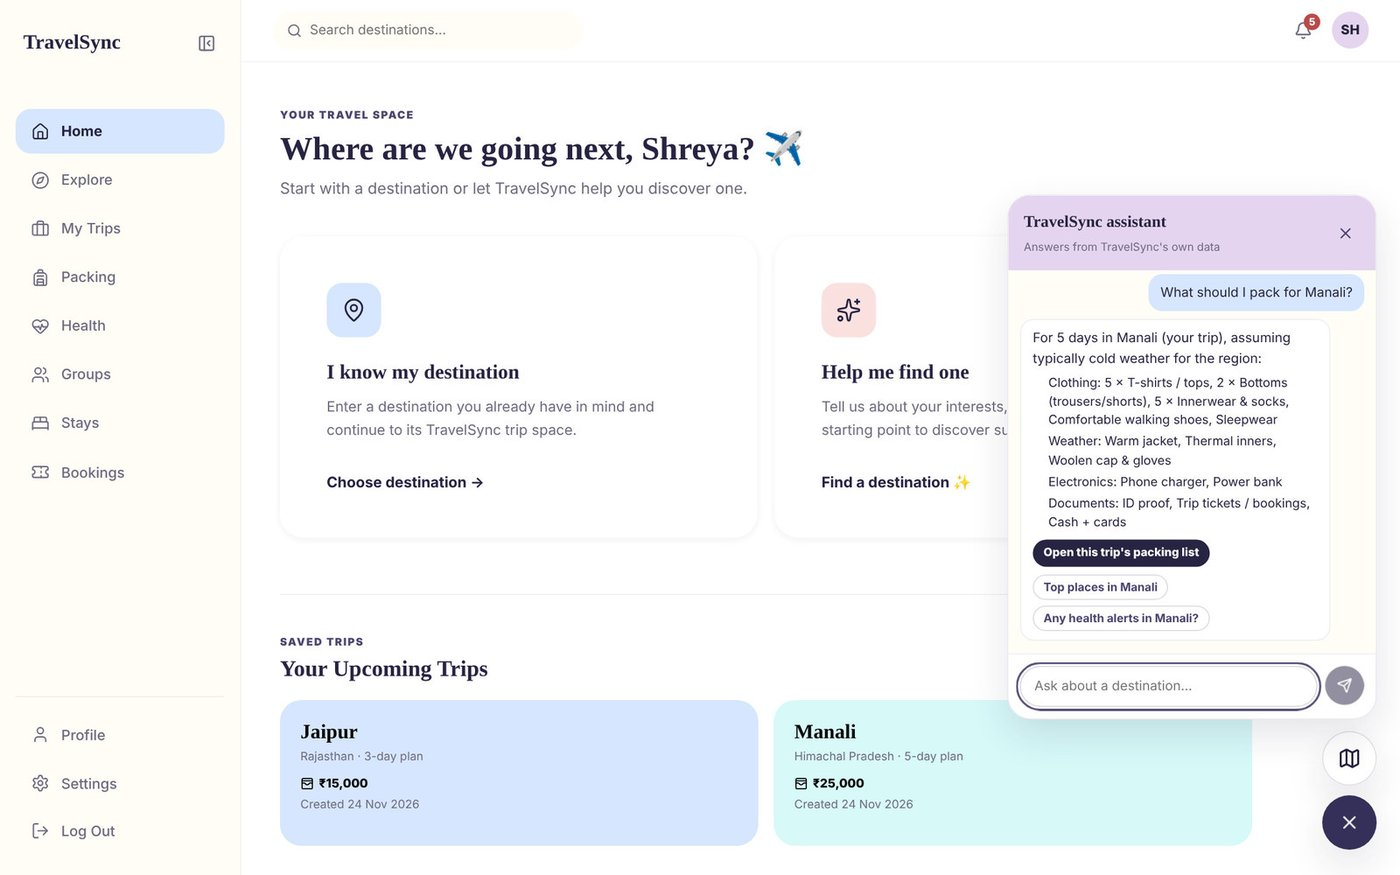
\includegraphics[width=0.9\textwidth]{screenshots/travel_assistant.jpg}
  \caption{TravelSync assistant answering a packing question}
  \label{fig:scr-assistant}
\end{figure}

\FloatBarrier

% ===== CHAPTER 3: RESULTS & EVALUATION =====

\chapter{Results and Evaluation}
\label{chap:results}

\section{Testing Methodology}

Testing was carried out continuously alongside development. Every feature
increment added or extended automated tests, and the full suites were run
before changes were merged. The testing strategy combined the following
levels \cite{pressman2015}:

\begin{itemize}
  \item \textbf{Unit Testing:} the rule-based engines and helpers were
    tested in isolation as pure functions: the password policy, the
    recommendation scoring functions, the packing checklist builder, the
    assistant's intent detection, file-type detection and the WebSocket
    chat hub on the backend, and the API client, input utilities, password
    policy and number fields on the frontend.
  \item \textbf{Integration Testing:} backend tests drive the complete
    FastAPI application through its HTTP and WebSocket interfaces with
    pytest \cite{pytest}, using an in-memory MongoDB-compatible database
    (mongomock-motor), so each test exercises routing, validation,
    authentication, authorisation, business logic and persistence together.
    External providers (Geoapify, Open-Meteo, SMTP and the optional language
    model) are replaced by controlled fakes that simulate success, timeouts,
    quota errors and malformed responses. Frontend tests render pages and
    components with Vitest \cite{vitest} and Testing Library in a jsdom
    browser environment against a mocked API.
  \item \textbf{Security Testing:} dedicated tests verify that every
    private endpoint rejects anonymous requests, that users cannot read,
    modify or delete another user's trips, bookings, files or groups, that
    tampered, expired and unsigned tokens are rejected, that cross-site
    state-changing requests are blocked, and that internal errors never leak
    database details.
  \item \textbf{Performance Testing:} response times of the main API
    endpoints and of the recommendation engine were measured on a running
    instance of the application, as reported in
    Section~\ref{sec:performance}.
  \item \textbf{User Testing:} the team carried out manual end-to-end
    walkthroughs of every workflow in the browser, including multi-user
    group sessions with four accounts. A formal usability study with
    external participants was not conducted within the project timeline and
    is listed as future work.
\end{itemize}

Table~\ref{tab:backend-tests} and Table~\ref{tab:frontend-tests} list the
automated test suites and the number of test cases in each.

\begin{table}[htbp]
\centering
\begin{tabular}{|l|L{0.33\textwidth}|r|}
  \hline
  \textbf{Test file} & \textbf{Area covered} & \textbf{Tests} \\
  \hline
  \texttt{test\_auth.py} & password policy, signup, login, sessions,
    tokens, recovery, CSRF and CORS & 36 \\
  \hline
  \texttt{test\_recommend\_stays\_health.py} & recommendation input
    validation, stays, health module & 28 \\
  \hline
  \texttt{test\_trips\_authorization.py} & trip ownership, validation,
    profile and settings & 21 \\
  \hline
  \texttt{test\_packing.py} & packing generation, edits, dates and
    forecast fallback & 20 \\
  \hline
  \texttt{test\_booking\_groups\_files.py} & group bookings and file
    attachments & 17 \\
  \hline
  \texttt{test\_chat\_assistant.py} & assistant intents and model
    fallback & 16 \\
  \hline
  \texttt{test\_bookings.py} & personal bookings & 14 \\
  \hline
  \texttt{test\_groups.py} & groups, chat, suggestions, voting,
    decisions & 14 \\
  \hline
  \texttt{test\_trip\_map.py} & map data and driving distances & 14 \\
  \hline
  \texttt{test\_chat\_socket.py} & live WebSocket delivery & 9 \\
  \hline
  \texttt{test\_chat\_delete.py} & deleting chat messages & 5 \\
  \hline
  \texttt{test\_chat\_history.py} & paging through chat history & 2 \\
  \hline
  \multicolumn{2}{|l|}{\textbf{Total (all passed)}} & \textbf{196} \\
  \hline
\end{tabular}
\caption{Backend test suites (pytest)}
\label{tab:backend-tests}
\end{table}

\begin{table}[htbp]
\centering
\begin{tabular}{|l|L{0.38\textwidth}|r|}
  \hline
  \textbf{Test file} & \textbf{Area covered} & \textbf{Tests} \\
  \hline
  \texttt{Bookings.test.jsx} & bookings page and files & 20 \\
  \hline
  \texttt{apiClient.test.js} & API client and errors & 15 \\
  \hline
  \texttt{utils.test.js} & shared utilities & 14 \\
  \hline
  \texttt{AppShell.test.jsx} & application shell & 13 \\
  \hline
  \texttt{RecommendDestination.test.jsx} & recommendation form & 12 \\
  \hline
  \texttt{GroupDetail.test.jsx} & group page & 7 \\
  \hline
  \texttt{Signup.test.jsx} & signup form & 6 \\
  \hline
  \texttt{ProfileMenu.test.jsx} & profile menu & 6 \\
  \hline
  \texttt{ChatWidget.test.jsx} & assistant widget & 5 \\
  \hline
  \texttt{ProtectedRoute.test.jsx} & route protection & 4 \\
  \hline
  \texttt{NumberField.test.jsx} & numeric input & 3 \\
  \hline
  \texttt{Login.test.jsx} & login form & 2 \\
  \hline
  \multicolumn{2}{|l|}{\textbf{Total (all passed)}} & \textbf{107} \\
  \hline
\end{tabular}
\caption{Frontend test suites (Vitest)}
\label{tab:frontend-tests}
\end{table}

Tables~\ref{tab:tc01}--\ref{tab:tc04} present the system-level test cases,
recorded in the test-case template prescribed for the course. They were
designed by the team and executed on 17 November 2026, and every step of all
four test cases passed.

% Course test-case template, page 1 of figures/test_cases.pdf
\begin{table}[htbp]
  \centering
  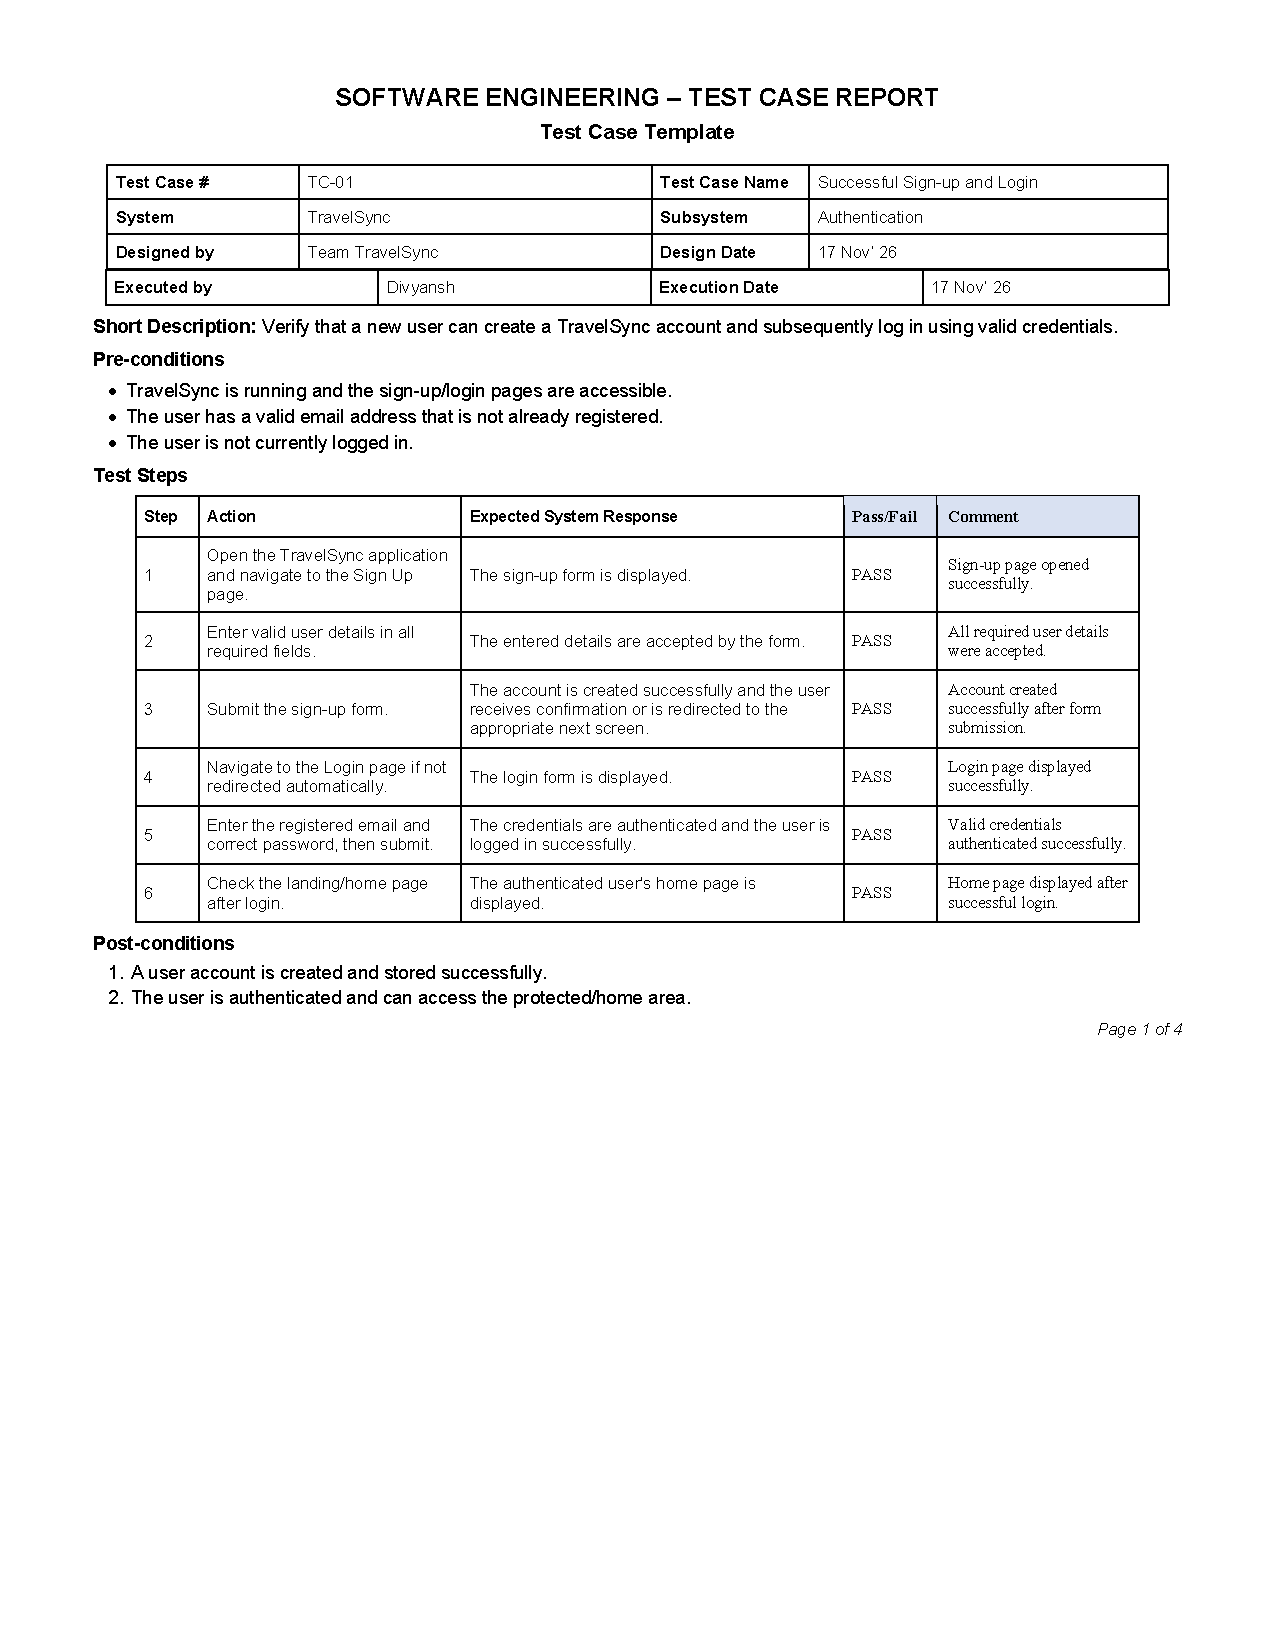
\includegraphics[page=1,width=\textwidth,trim=40 305 41 54,clip]{test_cases.pdf}
  \caption{Test case TC-01: Successful Sign-up and Login}
  \label{tab:tc01}
\end{table}

% Course test-case template, page 2 of figures/test_cases.pdf
\begin{table}[htbp]
  \centering
  \includegraphics[page=2,width=\textwidth,trim=40 288 41 54,clip]{test_cases.pdf}
  \caption{Test case TC-02: Destination Prediction}
  \label{tab:tc02}
\end{table}

% Course test-case template, page 3 of figures/test_cases.pdf
\begin{table}[htbp]
  \centering
  \includegraphics[page=3,width=\textwidth,trim=40 283 41 54,clip]{test_cases.pdf}
  \caption{Test case TC-03: Packing and Health Recommendations}
  \label{tab:tc03}
\end{table}

% Course test-case template, page 4 of figures/test_cases.pdf
\begin{table}[htbp]
  \centering
  \includegraphics[page=4,width=\textwidth,trim=40 319 41 54,clip]{test_cases.pdf}
  \caption{Test case TC-04: Top 5 Places and Stay Recommendations}
  \label{tab:tc04}
\end{table}

\section{Performance Metrics}
\label{sec:performance}

Response times were measured on a running instance of TravelSync on an
Apple MacBook Air (13-inch, 2025) with an Apple M4 processor (10 CPU cores)
and 16\,GB of memory, running macOS~26.5 and Python~3.14. The backend ran as a single Uvicorn worker process
with the in-memory MongoDB-compatible database employed by the test
suite and four registered users with trips, a group, chat messages,
suggestions, votes and bookings. Each endpoint was called 10 times to warm
up and then 200 times sequentially; login was measured over 20 calls.
Because the database ran in the same process, these figures measure the
application's own processing and exclude network latency to a MongoDB
server. Table~\ref{tab:performance} reports the results.

\begin{table}[htbp]
\centering
\begin{tabular}{|l|r|r|}
  \hline
  \textbf{Endpoint} & \textbf{Median} & \textbf{95th percentile} \\
  \hline
  \texttt{GET /api/health} & $0.5$\,ms & $0.6$\,ms \\
  \hline
  \texttt{GET /api/trips} & $0.7$\,ms & $0.7$\,ms \\
  \hline
  \texttt{GET /api/trips/\{id\}/packing-list} & $0.7$\,ms & $0.8$\,ms \\
  \hline
  \texttt{GET /api/groups/\{id\}/messages} & $0.8$\,ms & $0.9$\,ms \\
  \hline
  \texttt{GET /api/bookings} & $0.8$\,ms & $1.9$\,ms \\
  \hline
  \texttt{GET /api/places/\{destination\}} & $1.0$\,ms & $1.2$\,ms \\
  \hline
  \texttt{GET /api/destinations/search} & $1.0$\,ms & $1.1$\,ms \\
  \hline
  \texttt{POST /api/chat} & $1.4$\,ms & $1.4$\,ms \\
  \hline
  \texttt{POST /api/recommend} & $2.2$\,ms & $2.6$\,ms \\
  \hline
  \texttt{GET /api/travel-health/\{destination\}} & $5.2$\,ms & $5.4$\,ms \\
  \hline
  \texttt{POST /api/auth/login} & $167.7$\,ms & $168.4$\,ms \\
  \hline
\end{tabular}
\caption{API response times}
\label{tab:performance}
\end{table}

Throughput was measured on the same instance with 16 concurrent clients,
each sending requests back to back for 10 seconds per endpoint. The load
generator ran on the same laptop as the server, so the figures are a
conservative estimate for a single worker process. No request failed during
any run. Table~\ref{tab:throughput} reports the results.

\begin{table}[htbp]
\centering
\begin{tabular}{|l|r|r|}
  \hline
  \textbf{Endpoint} & \textbf{Throughput} & \textbf{Errors} \\
  \hline
  \texttt{POST /api/chat} & $830.8$\,req/s & $0$ \\
  \hline
  \texttt{GET /api/trips} & $740.8$\,req/s & $0$ \\
  \hline
  \texttt{GET /api/places/\{destination\}} & $730.4$\,req/s & $0$ \\
  \hline
  \texttt{GET /api/groups/\{id\}/messages} & $728.3$\,req/s & $0$ \\
  \hline
  \texttt{POST /api/recommend} & $491.2$\,req/s & $0$ \\
  \hline
  \texttt{GET /api/travel-health/\{destination\}} & $186.5$\,req/s & $0$ \\
  \hline
\end{tabular}
\caption{API throughput with 16 concurrent clients}
\label{tab:throughput}
\end{table}

The accuracy of the recommendation engine was measured as
\emph{precision at five} (Precision@5), the share of the top five
recommendations that are relevant to the request. For each of the twelve
interests, a request selecting only that interest at the highest importance
was issued once for each of the four traveller types (48 requests in total),
and a recommended destination was counted as relevant when its dataset score
for the selected interest was at least 0.5 on the 0--1 scale. Constraint
adherence and engine speed were measured separately over 300 randomly
generated requests from Ludhiana with random interests, importances,
traveller types, durations of 2 to 10 days, budgets from INR~10{,}000 to
INR~80{,}000 and maximum distances from 300 to 2{,}000\,km.
Table~\ref{tab:engine} summarises all evaluation metrics.

\begin{table}[htbp]
\centering
\begin{tabular}{|l|r|}
  \hline
  \textbf{Metric} & \textbf{Measured} \\
  \hline
  Precision@5 (relevance threshold 0.5) & $97.5\%$ (234 of 240) \\
  \hline
  Precision@5 (stricter threshold 0.7) & $86.3\%$ (207 of 240) \\
  \hline
  Top-ranked result relevant (threshold 0.5) & $100\%$ (48 of 48) \\
  \hline
  Relevant share of all destinations (random baseline) & $57.0\%$ \\
  \hline
  Recommendations within the stated maximum distance & $97.8\%$
    (1{,}508 of 1{,}542) \\
  \hline
  Recommendations within the 10\% distance tolerance & $100\%$ \\
  \hline
  Recommendations above 125\% of the stated budget & $0$ \\
  \hline
  Engine time per request, median / 95th percentile & $1.4$\,ms /
    $1.6$\,ms \\
  \hline
  Peak API throughput (one worker) & $830.8$\,req/s \\
  \hline
  Frontend JavaScript bundle (raw / gzip) & $448.0$\,kB / $129.8$\,kB \\
  \hline
  Automated tests passing (backend / frontend) & $196/196$ \,/\,
    $107/107$ \\
  \hline
\end{tabular}
\caption{Summary of evaluation metrics}
\label{tab:engine}
\end{table}

Precision@5 is reported instead of classification accuracy because a
recommender has no single correct answer for a request: a destination can
only be judged relevant or not relevant to it. All six non-relevant results
had a suitability score of at least 0.85 for the requested traveller type,
which shows the traveller-type weighting discussed in
Section~\ref{sec:analysis}.


\section{Analysis}
\label{sec:analysis}

\textbf{Did the project meet its objectives?} All four objectives were met.
Objective~1 is delivered by known-destination selection and the
recommendation engine, which returns explained rankings in a few
milliseconds and stays within the stated distance and budget limits.
Objective~2 is delivered by the trip workspace, which brings together the
top places, packing list, stays, health information and map for each trip.
Objective~3 is delivered by groups with invite codes, live chat, structured
suggestions, single-vote voting and an owner-confirmed decision.
Objective~4 is delivered by bookings with private files, upcoming and
previous trip views, notifications, the assistant, and the security model
verified by the authorisation tests.

\textbf{Where did the project exceed expectations?} The final system goes
beyond the mid-semester plan in several respects: live WebSocket delivery
with read receipts, unread counts and live voting updates; private file
attachments for bookings; a trip map with driving distances; trip editing;
password recovery; and a security design that includes token revocation,
login throttling, cross-site request checks and a production configuration
guard. A total of 303 automated tests pass, the recommender reaches a
Precision@5 of 97.5\%, and every interactive endpoint except deliberately
slow password hashing responds in under 6\,ms and sustains at least
186 requests per second on a single worker in the measured setting.

\textbf{What challenges were encountered?} The main challenges were:
\begin{itemize}
  \item \textbf{Free external-service quotas:} accommodation and routing
    providers limit daily requests, and live hotel prices are not available
    from open data.
  \item \textbf{Real-time consistency:} chat, votes and decisions must stay
    consistent when several members act at once or when a socket
    disconnects.
  \item \textbf{Concurrency and data integrity:} simultaneous requests could
    create duplicate packing lists, duplicate votes or an over-full group.
  \item \textbf{Ranking balance:} with a single interest selected, the fixed
    traveller-type weight can dominate the ranking; for Culture with the
    Solo type, the top five averaged a Culture score of 0.51, below the
    dataset mean of 0.62.
\end{itemize}

\textbf{How were they resolved?} Provider results are cached in MongoDB with
TTL indexes, live lookups are rate-limited per user, coordinates are rounded
before caching, and every provider failure degrades to a clear message or a
local fallback; prices are presented honestly as labelled estimates. Live
updates are sent only after the database write succeeds, and polling remains
as a fallback that catches up after a reconnection. Unique indexes and
atomic conditional updates enforce one packing list per trip, one vote per
member and the twenty-member group limit. The traveller-type weighting is
identified as a tuning target in Section~\ref{sec:future-work}.

The remaining limitations of the current version are that the chat hub keeps
socket connections in one process, so horizontal scaling would require a
shared message broker; that health alerts are curated by hand rather than
received from a live feed; that the recommendation weights were set by
design judgement rather than learned from user feedback; and that the
system has not yet been evaluated in a formal user study.

% ===== CHAPTER 4: CONCLUSION =====

\chapter{Conclusion}

\section{Summary of Work}

TravelSync set out to replace the fragmented, multi-application process of
planning a trip with a single platform. The team built a React single-page
application backed by an asynchronous FastAPI service and MongoDB, organised
around the idea that a chosen destination becomes a trip and every
supporting feature works from that trip.

All four objectives from Section~\ref{sec:objectives} were achieved. An undecided traveller
receives ranked, explained destination recommendations from a weighted
nearest-neighbour engine over 250 destinations that respects duration,
budget and distance constraints (Objective~1). Each trip opens a workspace
with its top places, a two-tier weather-aware packing list, scored
accommodation recommendations, historical health context and a map with
driving distances (Objective~2). Groups collaborate through invite codes,
live WebSocket chat, structured suggestions, one-member-one-vote voting and
an owner-confirmed decision (Objective~3). Bookings with private file
attachments, trip history, notifications and a privacy-preserving assistant
complete the platform, protected throughout by session security and per-user
authorisation (Objective~4). The system is covered by 303 passing automated
tests.

\section{Key Findings}

\begin{itemize}
  \item \textbf{Finding 1:} A transparent, content-based nearest-neighbour
    ranking combined with simple constraint scores was sufficient for
    destination recommendation without any training data. The engine
    reached a Precision@5 of 97.5\% against a random baseline of 57\%,
    answered each request in under 2\,ms, and never violated the budget
    ceiling or the distance tolerance.
  \item \textbf{Finding 2:} Designing every external dependency to fail
    gracefully, through caching, per-user limits and local fallbacks, made
    it possible to build on free-tier services while keeping the application
    usable when a provider was slow, exhausted or unavailable.
  \item \textbf{Finding 3:} The evaluation exposed an unexpected interaction
    in the ranking: the fixed weight given to the traveller type can
    outweigh a single selected interest, so that for some combinations (for
    example Culture with the Solo type) the recommendations favour the
    traveller-type profile over the interest itself.
\end{itemize}

\section{Future Work and Recommendations}
\label{sec:future-work}

The current version provides a complete foundation that can be extended in
the following directions:

\begin{enumerate}
  \item Potential enhancements to the system: tune the traveller-type
    weight and the final-score weights using recorded user choices, so that
    the recommender learns from which destinations users actually select
    \cite{lops2011content}.
  \item Alternative approaches worth exploring: combine the content-based
    engine with collaborative filtering once enough trips have been
    recorded, and replace the hand-curated health alerts with an automated
    feed from official surveillance sources \cite{idsp}.
  \item Scalability improvements: move the in-process chat hub to a shared
    message broker so that several backend workers can serve WebSocket
    clients, and move booking files to object storage as their volume grows.
  \item Integration with other systems: link TravelSync with transport and
    hotel providers that publish real prices and availability, and allow
    itineraries to be exported to calendar applications.
  \item Real-world deployment considerations: conduct a formal usability
    study, add multilingual support, and complete a production deployment
    with HTTPS, monitoring and automated backups of the MongoDB database.
\end{enumerate}

\section{Final Remarks}

Building TravelSync gave the team practical experience of the complete
software engineering life cycle: turning a proposal into requirements and
UML models, revising the design when implementation revealed better options
(such as replacing a planned administrator role with versioned datasets, and
a separate messaging service with native WebSockets), and validating the
result with automated tests and measurements. The most valuable lessons
were the importance of explainable algorithms that can be defended to users
and evaluators, of security and authorisation designed in from the first
increment rather than added at the end, and of honest presentation of data,
such as labelling estimated prices and historical health information for
what they are. The resulting platform demonstrates that discovery,
preparation and group coordination for a trip can be brought together in one
coherent and trustworthy experience.


% ===== BIBLIOGRAPHY =====

% Print bibliography with heading in TOC
\printbibliography[heading=bibintoc]

\end{document}
